%%%%%%%%%%%%%%%%%%%%%%%%%%%%%%%%%%%%%%%%%%%%%%%%%%%%%%%%%%%%%%%%%%%%%%%%%%%%%
%% obtained from https://canvas.uva.nl/courses/6063/files/folder/Templates %%
%%%%%%%%%%%%%%%%%%%%%%%%%%%%%%%%%%%%%%%%%%%%%%%%%%%%%%%%%%%%%%%%%%%%%%%%%%%%%
\documentclass{uvamath}
\usepackage[english]{babel}


\usepackage{graphicx}
\graphicspath{{assets/}}
\usepackage{listings}
\usepackage{scrhack} % required for listings to work with KOMA script document class
\usepackage{graphbox}
\usepackage{amssymb}
\usepackage{amsmath}
\usepackage{amsthm}
\usepackage{stmaryrd} % For llbracket, rrbracket
\usepackage[pdfborder={0 0 0}]{hyperref}
\hypersetup{colorlinks=true, linkcolor=blue}

\usepackage{csquotes,xpatch} % Recommended by biblatex
\usepackage[style=numeric]{biblatex}
\addbibresource{zotero.bib}
\addbibresource{manual.bib}

\usepackage[a4paper, nohead]{geometry}

% Load custom macros
\newcommand{\N}{\mathbb{N}}
\newcommand{\R}{\mathbb{R}}

% Flag Images

\newcommand{\edge}{{\includegraphics[align=c,scale=0.5]{flags/edge.pdf}}}
\newcommand{\nonedge}{{\includegraphics[align=c,scale=0.5]{flags/nonedge.pdf}}}

\newcommand{\triangleflag}{{\includegraphics[align=c,scale=0.5]{flags/k3.pdf}}}
\newcommand{\triangleoneedge}{{\includegraphics[align=c,scale=0.5]{flags/k3-1edge.pdf}}}
\newcommand{\triangletwoedge}{{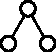
\includegraphics[align=c,scale=0.5]{flags/k3-2edge.pdf}}}
\newcommand{\triangleempty}{{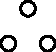
\includegraphics[align=c,scale=0.5]{flags/k3-empty.pdf}}}

\newcommand{\kfour}{{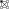
\includegraphics[align=c,scale=0.5]{flags/k4.pdf}}}
\newcommand{\cfour}{{\includegraphics[align=c,scale=0.5]{flags/c4.pdf}}}
\newcommand{\kfourbucket}{{\includegraphics[align=c,scale=0.5]{flags/k4-bucket.pdf}}}
\newcommand{\kfourtwopair}{{\includegraphics[align=c,scale=0.5]{flags/k4-2pair.pdf}}}
\newcommand{\kfourmone}{{\includegraphics[align=c,scale=0.5]{flags/k4m1.pdf}}}
\newcommand{\kfourmtwo}{{\includegraphics[align=c,scale=0.5]{flags/k4m2.pdf}}}

\newcommand{\cfive}{{\includegraphics[align=c,scale=0.5]{flags/c5.pdf}}}


\title{Local Flags: Bounding the Strong Chromatic Index} % Title of your thesis
\author[eoin.davey@student.uva.nl, 14246287]{Eoin Davey} %Your name, email and student number

\documentTitle{Master Thesis}
\program{MSc Mathematics} % MSc Mathematics / MSc Mathematical Physics / Stochastics and Financial Mathematics

\supervisorsTitle{Dr. J.R. Kang} %This is the list of supervisors for the title page, seperate with \newline

\supervisors{Dr. J.R. Kang} %This is the list of supervisors for the second page, seperate with comma

\secondexaminer{Dr. K. Guo} %This is the name of the second examiner, for the second page
\date{June 28, 2024} %This is the examination date, i.e. the date of your thesis presentation

\newtheorem{theorem}{Theorem}[chapter]
\newtheorem{lemma}[theorem]{Lemma}
\newtheorem*{knownlemma}{Lemma}
\newtheorem{corollary}{Corollary}[theorem]
\newtheorem*{knowntheorem}{Theorem}
\newtheorem{conjecture}{Conjecture}[chapter]
\newtheorem*{knownconjecture}{Conjecture}
\newtheorem{note}{Note}[section]
\newtheorem*{note*}{Note}
\newtheorem{definition}{Definition}[chapter]
\newtheorem*{example}{Example}

\begin{document}
\newgeometry{margin=1in}
\maketitle
\restoregeometry

\begin{abstract}
    In this thesis we introduce a novel framework inspired by Razborov's flag algebras
    which we are calling \textit{local flags}. This new framework enables us to use
    the semidefinite method to prove new bounds on a wide family of "local" combinatorial
    functions. We use this new framework to
    make progress on a conjecture of Erd\H{o}s and Nešetřil, finding a
    best-yet asymptotic upper bound on the strong chromatic index of a graph.
    We also apply this new framework to make the first progress on the bipartite special case of
    this conjecture.
    Additionally, we explore a bounded degree version of Erd\H{o}s' pentagon
    conjecture: We state a conjecture and make significant progress toward proving it using
    the new framework. This thesis serves as both an introduction and a handbook on applying
    this method as we believe it has the potential to be used for many other applications.
\end{abstract}

\setcounter{tocdepth}{1}
\newgeometry{margin=1in}
\tableofcontents
\restoregeometry

\chapter*{Introduction}
\addcontentsline{toc}{chapter}{Introduction}

Consider a simple\footnote{An undirected graph with no self loops and at most 1 edge between any two
vertices.} graph $G$. How many colours do you need to colour each edge such that no edges which touch
have the same colour? What if no edges which touch some common edge can have the same colour?
Erd\H{o}s and Nešetřil conjectured that you only need $1.25\Delta(G)^2$ colours but
the best known proof only shows an upper bound of $1.772\Delta(G)^2$ colours. In this thesis
we show how we can bring this bound down to $1.73\Delta(G)^2$ by introducing a novel framework
which is a modification of Razborov's flag algebras. We also apply this new framework
to some other open problems including a bounded-degree version of the
Erd\H{o}s' pentagon conjecture.

\section*{Strong Edge Colouring}
\addcontentsline{toc}{section}{Strong Edge Colouring}
\label{sec:intro_strong_edge_coloring}

An edge colouring of a simple graph $G$ is an assignment $c\colon E(G) \to [k]$
for some $k\in\N$. Such a colouring is \textit{proper} if no two incident\footnote{Have a vertex in common}
edges have the same colour.
A colouring is \textit{strong} if no edges which share a common incident edge have
the same colour. Put differently, proper colouring requires edges at distance 1 to have distinct
colours and strong colouring extends this to distance 2.
In figure \ref{fig:proper-strong-example} we see an example of a non-proper colouring,
a proper (but not strong) colouring and a strong colouring of $C_5$.

\begin{figure}[h]
    \centering
    \includegraphics[scale=1.5]{proper-strong-example}
    \caption{Non-Proper, Proper \& Strong Edge Colourings}
    \label{fig:proper-strong-example}
\end{figure}

The \textit{chromatic index} of $G$, denoted $\chi'(G)$, is the minimum $k$ such that a proper edge
colouring of $G$ with $k$ colours exists. The \textit{strong chromatic index} $\chi'_s(G)$
is the corresponding minimum number of colours required for a strong edge colouring.

Vizing's theorem is a well known result which tells us $\chi'(G)$ almost exactly in terms of
the max degree of the graph $\Delta(G)$:
\begin{knowntheorem}[Vizing, 1965 \cite{Vizing_1965}]
    $\Delta(G) \leq \chi'(G) \leq \Delta(G) + 1$.
\end{knowntheorem}
Erd\H{o}s and Nešetřil conjectured in 1985 that
the strong chromatic index can also be bounded precisely by a function of the max degree:
\begin{knownconjecture}[Erd\H{o}s and Nešetřil \cite{faudreeInducedMatchingsBipartite1989}]
    \label{conj:intro_erdos_nesetril}
    $\chi'_s(G) \leq \frac{5}{4}\Delta(G)^2$.
\end{knownconjecture}
A greedy argument shows a bound of $\chi'(G) \leq 2\Delta(G)^2 + o(\Delta(G)^2)$ but it wasn't until
1997 that Molloy and Reed broke the $2\Delta(G)^2$ barrier \cite{molloyBoundStrongChromatic1997}.
A series of papers have since made progress on bringing this bound down closer to $\frac{5}{4}\Delta(G)^2$.

For $\Delta(G)$ large enough we have the following theorems:
\begin{enumerate}
  \item \textit{Molloy \& Reed, 1997} \cite{molloyBoundStrongChromatic1997}:
        $\chi'_s(G) \leq 1.998\Delta(G)^2$.
  \item \textit{Bruhn \& Joos, 2015} \cite{bruhnStrongerBoundStrong2018}:
        $\chi'_s(G) \leq 1.93\Delta(G)^2$.
  \item \textit{Bonamy, Perrett \& Postle, 2018} \cite{bonamyColouringGraphsSparse2018}:
        $\chi'_s(G) \leq 1.835\Delta(G)^2$.
  \item \textit{Hurley, de Verclos \& Kang, 2022} \cite{hurleyImprovedProcedureColouring2022}:
        $\chi'_s(G) \leq 1.772\Delta(G)^2$.
\end{enumerate}

In this thesis we will show how we brought this bound down even further to $1.73\Delta(G)^2$:
\begin{knowntheorem}
    For $\Delta(G)$ large enough we have
    $\chi'_s(G) \leq 1.73\Delta(G)^2$.
\end{knowntheorem}

The 1997 paper by Molloy \& Reed introduced a method for strong edge colouring we call the
\textit{2 step strategy}:
\begin{enumerate}
    \item Find an upper bound for the \textit{strong neighbourhood density} of $G$ in terms of
        $\Delta(G)$.
    \item Use a probabilistic colouring method which uses the previous bound to achieve a colouring
        with a low number of colours.
\end{enumerate}
This method has been modified by the papers which followed the Molloy \& Reed paper but this
strategy has remained the core idea. We will look at this strategy in more detail (including
defining strong neighbourhood density) in chapter \ref{chap:strong_edge_colouring}.
For this thesis we focus on the first step, using the second step as a black box. We will
find a new, lower, upper-bound on the strong neighbourhood density and hence achieve our
new colouring number.

\section*{Flag Algebras}
\addcontentsline{toc}{section}{Flag Algebras}

Step 1 of the 2-step strategy
asks us to find an upper bound on the strong neighbourhood density. The strong neighbourhood
density belongs to a broad family of density functions which ask: "How many copies of some
structure $F$ do we find in some larger structure $G$, expressed as a real number $\in [0,1]$"?
These density functions usually count the number of copies of $F$ in $G$, then normalise by the
maximum possible number of such copies.
For example, the density of edges in some graph $G$ is $|E(G)|/\binom{|G|}{2}$.

Bounding densities
is a common problem in combinatorics and in 2007 Razborov \cite{razborovFlagAlgebras2007}
introduced a framework called \textit{flag algebras}
which can be used to prove asymptotic results about densities in various combinatorial settings.
These flag algebras are defined very generally in terms of finite model theory in \cite{razborovFlagAlgebras2007} but we focus on their use with respect to simple graphs.

We give a brief flavour of flag algebras here but defer a full exposition until
chapter \ref{chap:classic_flags}.

\subsection*{A motivating example}
\label{sec:motivating_example}

As a reminder, for a graph $G$ and subset of vertices $U\subseteq V(G)$ the \textit{induced subgraph}
$G[U]$ is the subgraph of $G$ consisting of the vertices in $U$ and all edges between them.
We can then define the \textit{induced count} of $F$ in $G$, denoted $c(F; G)$, as
the number of subsets $U\subseteq V(G)$ such that $G[U] \cong F$. Then we define the
\textit{induced density} as $p(F; G) := c(F; G) / \binom{|G|}{|F|}$.

\begin{note}
    $p(F; G)$ is precisely the same as the probability that $G[U] \cong F$ if
    $U \subseteq V(G)$ is a uniformly random subset of size $|F|$.
\end{note}

What are some simple algebraic relationships between small subgraphs?
One thing that seems intuitive is that the density of edges in $G$ plus the density
of non-edges in $G$ is precisely 1. Similarly the densities of all possible graphs on
3 vertices is also 1.
\begin{align*}
    p(\edge; G) + p(\nonedge; G) &= 1\\
    p(\triangleflag; G)
    + p(\triangletwoedge; G)
    + p(\triangleoneedge; G)
    + p(\triangleempty; G) &= 1
\end{align*}

The density of edges is the probability that if we pick a pair of vertices that there is an
edge between them. We can relate this to the densities of graphs on 3 vertices by remarking
that sampling a pair of vertices uniformly at random can be done by first sampling a
triple of vertices at random, and then sampling 2 of those 3 uniformly again. This gives
us the following relation:
\[
    p(\edge; G) = 
    p(\triangleflag; G)
    + \frac{2}{3}p(\triangletwoedge; G)
    + \frac{1}{3}p(\triangleoneedge; G)
    + 0\cdot p(\triangleempty; G)
\]
A similar thought experiment relating sampling two pairs uniformly at random to sampling 4
vertices and then splitting the 4 randomly into two halves tells us:
\[
    p(\edge; G)^2 \sim p(\kfour; G) + \frac{2}{3}\left(p(\kfourmone; G) + p(\cfour; G)\right)
        + \frac{1}{3}\left(p(\kfourmtwo; G) + p(\kfourbucket; G) + p(\kfourtwopair; G)\right)
\]

Simplifying our notation then we might arrive at a symbolic algebra which has relations
like
\begin{align*}
    \edge + \nonedge &= 1\\
    \triangleflag
    + \triangletwoedge
    + \triangleoneedge
    + \triangleempty &= 1\\
    \edge &=
    \triangleflag
    + \frac{2}{3}\triangletwoedge
    + \frac{1}{3}\triangleoneedge\\
    \edge^2 &=
    \kfour + \frac{2}{3}(\kfourmone + \cfour)
        + \frac{1}{3}(\kfourmtwo + \kfourbucket + \kfourtwopair).
\end{align*}

We can then prove results with simple symbolic manipulation: In a triangle free graph
we would have $\triangleflag = 0$, hence
\[
    \edge = \frac{2}{3}\triangletwoedge + \frac{1}{3}\triangleoneedge \leq
    \frac{2}{3}(\triangletwoedge + \triangleoneedge)
    \leq \frac{2}{3}(\triangleflag + \triangletwoedge + \triangleoneedge + \triangleempty)
    \leq \frac{2}{3}
\]
as flags are non-negative. This (given all the formal definitions and proofs we've deferred)
is a formal proof
that $p(\edge; G) \leq \frac{2}{3}$ for any triangle free graph. The best possible result
says that $p(\edge; G) \leq \frac{1}{2}$ and is known as
\textit{Mantel's theorem} \cite{Mantel_1910}. This is
also easily proved with flag algebras which is seen in chapter \ref{chap:classic_flags}.

\subsection*{Computer Search}

One of the most (if not \textit{the most}) important aspects of flag algebras is that
they lend themselves very well to computer search methods.
The flag algebras allow us to prove results using only simple symbol manipulation in a very
tractable way; All details of the structures at play are abstracted out, only algebraic relations
between real numbers remains. We then have several tools at our disposal, in particular
linear combinations of flag inequalities can capture complex counting arguments, and
we will see later an operator on the algebra which enables us to use Cauchy-Schwarz style
arguments.

In practice we use the \textit{semidefinite method} to optimise some objective function
over the algebra, and due to duality this gives us a rigorous proof of an upper bound on our
function.
We will see in section \ref{sec:semidefinite_method} how we construct the semidefinite program,
and how we can interpret the dual solutions in a more human understandable way.

\section*{Local Flags}
\addcontentsline{toc}{section}{Local Flags}

One might be tempted to try to apply these flag algebras directly to our strong neighbourhood
density problem but in practice this problem doesn't fit well into the flag algebra model.
In particular, Razborov's flag algebras are constructed to work well with density functions
like the induced density function $p(F; G) = c(F; G)/\binom{|G|}{|F|}$ which have a
denominator which is $\Theta(|G|^{|F|})$. This is convenient if we are trying to prove
a bound on some function which is polynomial in $|G|$
(e.g. Mantel's theorem says the number of edges is $\leq \frac{1}{4}|G|^2$). But what if
we want to prove a bound on a function which is polynomial in some other function
of $G$? e.g. The \hyperref[conj:intro_erdos_nesetril]{Erd\H{o}s-Nešetřil Conjecture}
wants to bound $\chi'_s(G)$ with a polynomial in $\Delta(G).$ This does not lend itself
to the same methods.

Instead, we can define a new "density" function which instead normalises our induced
count by a different denominator, one which captures the graph parameter we want to measure
our count "relative to". In particular, in chapter \ref{chap:local_flags} we introduce a
new \textit{local density function} and a concept we call a \textit{local flag}.
We show that, under certain conditions, these local flags also form a nice algebra
with which we can apply the semidefinite method to prove bounds. We then apply this new
method to several problems, including the 
\hyperref[conj:intro_erdos_nesetril]{Erd\H{o}s-Nešetřil Conjecture}.

\section*{Contributions}
\addcontentsline{toc}{section}{Contributions}

The concept for this new framework was originally explored by \textit{de Verclos} in
2020\footnote{In unpublished notes}.
They conjectured the structure of the framework, then adapted flag algebra
software\footnote{\url{https://crates.io/crates/flag-algebra}}
to test if this framework could in principle improve on existing results.
This experiment showed that if the framework could be realised formally then it could improve the
best known bound on the strong chromatic index.
The contribution of chapter \ref{chap:local_flags} is the concretisation of this idea:
We give original definitions, results and proofs which make this framework rigorous.

Using this new framework we have made progress on several open problems:
\begin{itemize}
    \item In chapter \ref{chap:pentagon_conjecture} we show a "warmup" application of the new
        framework. We make a new conjecture which is a bounded degree version of the famous
        Erd\H{o}s pentagon conjecture \cite{erdos_pentagon_1984}.
        We show then how a straightforward application of the local flags method makes non-trivial
        progress towards proving the conjecture, and show that a slightly more complex application
        then gets even closer to the full result.
        This problem was chosen as the original conjecture was first proven using
        the classic flag algebras (\cite{hatamiNumberPentagonsTrianglefree2013},
        \cite{grzesikMaximumNumberFivecycles2012}).
    \item In chapter \ref{chap:strong_edge_colouring} then we apply this new framework to make progress on the
        \hyperref[conj:intro_erdos_nesetril]{Erd\H{o}s-Nešetřil Conjecture}, achieving the best-yet
        bound of $\chi'_s(G) \lesssim 1.73\Delta(G)^2$. The approach used here is a modification
        of the approach conjectured by de Verclos.
    \item At the end of chapter \ref{chap:strong_edge_colouring} we alter the method to make
        the first progress on the special bipartite version of this conjecture, showing that
        if $G$ is bipartite then we have the bound $\chi'_s(G) \lesssim 1.6254\Delta(G)^2$.
\end{itemize}


\chapter{Background: Classic Flag Algebras}
\label{chap:classic_flags}

In section \ref{sec:flag_algebras} we will briefly introduce Razborov's
flag algebras as they apply to
graphs. If the reader is already familiar with flag algebras this section can be skipped.

In section \ref{sec:semidefinite_method} we will discuss how the semidefinite method is applied
to flag algebras.
The method we use is slightly different to the method used in other works
(e.g. \cite{silvaFlagAlgebrasFirst2016}) but is more easily adapted to our new framework. This
section may be of interest even to a reader familiar with flag algebras.

Finally in section \ref{sec:coloured_graphs} we will introduce \textit{coloured graphs} as combinatorial
objects with their own structure. These will help us unlock the full potential of
our local flags in section TODO.

\section{Flag Algebras}
\label{sec:flag_algebras}

All the following definitions, theorems etc.
are concepts from \cite{razborovFlagAlgebras2007}, rephrased
to focus only on the simple graph case.
For similar introductions to flag algebras we point the reader to
\textit{Flag Algebras: A First Glance} by Silva, Filho and Sato
\cite{silvaFlagAlgebrasFirst2016} and \textit{A Brief Introduction to Flag Algebra} by Qi
\cite{qiBriefIntroductionFlag}.

We saw in the \hyperref[sec:motivating_example]{motivating example} above that we want
to construct a symbolic algebra out of small graphs with some nice properties:
\begin{itemize}
    \item We would like the algebraic operations
        to be easily computable\footnote{at least with some computer software assistance}.
    \item We want the algebra to describe true relationships about densities in large graphs.
        i.e. If $A + B \geq C^2\cdot D$ is a true statement in our algebra
        then that must imply that $p(A; G) + p(B; G) \geq p(C; G)^2 \cdot p(D; G)$ for any $G$ large
        enough.
\end{itemize}

When we defined the induced count $c(F; G)$ we counted all possible instances of $F$
in $G$; Sometimes we want to only consider a subset of those instances, those where
we force some fixed vertices in $F$ to be mapped to some fixed vertices in $G$.
(e.g. if we count the copies of $\edge$ in $G$ where we force the first vertex to be mapped
to some fixed $v\in V(G)$ then $c(F; G) = \deg v$). This motivates the last desirable
properties of our algebra.

\begin{itemize}
    \item We would like our symbolic algebra to be able to capture densities where we have fixed
        some vertices.
    \item We want to be able to relate these "fixed" densities to the un-fixed densities.
\end{itemize}

Razborov's flags algebras give us all these nice properties. This section covers the
basic formalisms; Introducing a density function which accounts for pre-fixing some vertices,
defining what it means for something to hold "for large graphs", defining the actual
flag algebras with their properties, introducing an ordering $\geq$ and finally
covering the averaging operator which
relates "fixed vertex" densities to their un-fixed counterparts.

\subsection{Flags}

The fundamental object of our algebra is the \textit{flag} which is a partially
labelled graph, meaning some of the vertices of the graph have integer labels assigned to
them\footnote{The term flag apparently refers to the fact that some of the graph is fixed and the rest hangs loose, like a flag in the wind}. There may be no labelled vertices.
The labelled vertices will correspond then to those vertices which are fixed when we count
copies of the graph in some larger graph.

The \textit{type} of the flag is the subgraph induced by the labelled vertices.
In figure \ref{fig:flags-types} we see some example flags and their types. The labelled vertices
are represented visually with a partially filled vertex.

\begin{figure}[h]
    \centering
    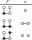
\includegraphics{flags-types-example}
    \caption{Example flags and their types}
    \label{fig:flags-types}
\end{figure}

We give the formal definitions:

\begin{definition}[Type]
    \label{def:type}
    A \textbf{type} $\sigma$ of size $k$ is a graph with vertex set $[k]$. We write
    $|\sigma|$ to denote the size of the underlying graph. We write
    $\emptyset$ to denote the type consisting of the empty graph.
\end{definition}
\begin{definition}[$\sigma$-Embedding]
    Given a type $\sigma$ and a graph $F$, a \textbf{$\sigma$-embedding} is an injective
    function $\theta\colon[|\sigma|]\to V(F)$ which is a graph isomorphism between
    $\sigma$ and $F[\im \theta]$.
\end{definition}
\begin{definition}[$\sigma$-Flag]
    \label{def:sigma_flag}
    A \textbf{$\sigma$-flag} is a tuple $(F, \theta)$ where $\theta$ is an $\sigma$-embedding
    into $F$.
    If the embedding is implicit (e.g. if $\sigma=\emptyset$) we often drop the
    $\theta$ from the notation.
\end{definition}

\begin{note}
    A type $\sigma$ is implicitly itself a $\sigma$-flag when taken with the
    identity embedding $\id\colon [|\sigma|] \to [|\sigma|]$. We often use this fact
    implicitly.
\end{note}

We then say that two flags are isomorphic if there is a graph isomorphism between the underlying
graphs which preserves the labels.
\begin{definition}[Flag Isomorphism]
    $f\colon V(F) \to V(F')$ is a $\sigma$-flag isomorphism
    from $(F,\theta) \to (F', \theta')$ if it is graph isomorphism $F \to F'$ such that
    $f(\theta(i)) = \theta'(i)\ \forall\ i\in [|\sigma|].$ We can
    write $(F,\theta)\cong (F',\theta')$ if such an $f$ exists.
\end{definition}

Now that we have a definition for flags we can build on our induced density function from
the introduction.

\subsection{Induced Counts and Density}

In the introduction we defined the induced count $c(F; G)$ to be the number of
$U\subseteq V(F)$ such that $G[U] \cong F$. If both $F$ and $G$ are partially labelled
and have the same type (so are "compatible"), then we
can ask how many copies of $F$ are there in $G$ where the fixed part of $F$ maps to the
fixed part in $G$.

\begin{definition}[Induced Count]
    \label{def:induced_count}
    Fix two $\sigma$-flags $(F,\theta), (G,\eta).$ We define the induced count of $(F,\theta)$ in
    $(G,\eta)$ written $c((F,\theta); (G,\eta))$
    as the number of subsets $\im(\eta)\subseteq U\subseteq V(G)$ such that
    $(F,\theta) \cong (G[U], \eta)$.\footnote{Where we restrict the codomain of $\eta$ appropriately}
\end{definition}

We can extend this notion of counting how many copies of $F$ there are in $G$ to multiple flags,
asking how many tuples of disjoint copies of $F_1, \dots, F_t$ are there in $G$ (where
disjoint means vertex-disjoint apart from the fixed labelled vertices).

Precisely we define $c(F_1, \dots, F_t; G)$ to be the number of
$U_1, \dots, U_t\subseteq V(G)$ such that $\im\eta = U_i \cap U_j\ \forall\ i, j \in [t]$ where
$i\neq j$ and $(F_i, \theta_i) \cong (G[U_i], \eta)$ for all $i\in [t].$

Note that if $c(F_1, \dots, F_t; G) > 0$ we know that $G$ must be large enough to fit
disjoint copies of $F_1, \dots, F_t$ leading us to the following definition.

\begin{definition}[Fit]
    We say $\sigma$-flags $F_1, \dots, F_t$ \textbf{fit} in $\sigma$-flag $G$ if
    $|G|-|\sigma| \geq \sum_{i=1}^t |F_i|-|\sigma|$.
\end{definition}

\begin{example}
    Consider the type $\sigma=\vertex$, a single vertex. Any $\sigma$-flag $(G,\eta)$ is
    just a graph with a specific distinguished vertex (the unique labelled vertex).

    Consider then the $\sigma$-flag $F=\edgemarked$, an edge with a single labelled vertex.
    For any $G$ with distinguished vertex $v$ we have $c(\edgemarked; G^v) = \deg_G(v)$.
    \footnote{$G^v$ is the $\vertex$-flag $(G,\theta)$ where $\theta(1)=v$.}

    Similarly, $c(\edgemarked, \edgemarked; G^v) = \binom{\deg(v)}{2}.$ This is as
    we are counting how many distinct pairs of vertices $(a, b)$ are there in $G$ such that
    $G[\{a, v\}] \cong \edgemarked$ and $G[\{b, v\}] \cong \edgemarked$.
    In other words, how many distinct pairs of vertices are there connected to
    $v$, which is clearly $\binom{\deg(v)}{2}.$
\end{example}

Now we can define the induced density by normalising the induced count by the max
possible number of such non-overlapping $t$-tuples.

\begin{definition}[Induced Density]
    \label{def:induced_density}
    Given $\sigma$-flags $F_1, \dots, F_t$ and $G$ define the \textbf{induced density} of
    $F_1, \dots, F_t$ in $G$ as:
    \[
    p(F_1, \dots, F_t; G)
    := \frac{c(F_1, \dots, F_t; G)}{
    \binom{|G|-|\sigma|}{|F_1|-|\sigma|, \dots,|F_t|-|\sigma|, R}}
    \]
    where we use multinomial coefficient notation with
    $R=(|G|-|\sigma|)-\sum_{i=1}^t |F_i|-|\sigma|$.
\end{definition}

\begin{note}
    Again, as in the \hyperref[sec:motivating_example]{motivating example in the introduction},
    we can interpret $p(F_1, \dots, F_t; G)$ in a precise probabilistic way.
    $p(F_1, \dots, F_t; G)$ is exactly the probability that
    $(F_i, \theta_i) \cong (G[U_i], \eta)\ \forall\ i\in[t]$ where
    $U_1, \dots, U_t \subseteq V(G)$ is a uniformly random $t$-tuple of subsets such that
    $U_i \cap U_j = \im \eta\ \forall i, j \in [t], i \neq j$.
\end{note}

\subsection{Graph Classes}

Often, we want to limit our view to a subset of all possible graphs. For example, we
will want to consider only triangle-free graphs when proving Mantel's theorem (TODO REF).

We pick some class of graphs $\Gcl$. For Razborov's flag algebras we assume that
$\mathcal{G}$ is hereditary, meaning it is closed under taking induced subgraphs. This will change
when we introduce our new local framework.

Then for any type $\sigma$ we write $\Gcl^\sigma$ for the set of all $\sigma$-flags up to
isomorphism. We write $\Gcl^\sigma_n$ for the set of all $\sigma$-flags of size $n$.
We generally assume $\Gcl^\sigma$ is infinite for any type $\sigma\in\mathcal{G}$.
If $\sigma=\emptyset$ we often skip the superscript and just refer to
$\Gcl$ or $\Gcl_n$.

From this point all definitions and results are relative to some fixed graph class
$\mathcal{G}$.

Given some graph class $\mathcal{G}^\sigma$ then we get the very power \textit{chain rule}.
\begin{lemma}[The Chain Rule, Lemma 2.2 \cite{razborovFlagAlgebras2007}]
    \label{lemma:chain_rule}
    If $F_1, \dots, F_t \in \Gcl^\sigma$ are $\sigma$-flags which fit in $G\in\Gcl^\sigma$
    then for all $1 \leq s \leq t$ and every $n$ such that
    $F_1, \dots, F_s$ fit into a $\sigma$ flag of size $n$ and a
    $\sigma$-flag and $F_{s+1}, \dots, F_t$ fit in $G$ we have:
    \[
    p(F_1, \dots, F_t; G) = \sum_{F \in \mathcal{G}^\sigma_n}
    p(F_1, \dots, F_s; F)p(F, F_{s+1}, \dots, F_t; G).
    \]
\end{lemma}

This chain rule is one of the crucial properties that we will lose when we define our
local flags framework.

\subsection{Limit Functionals}
\label{sec:limit_functionals}

We want to define our algebra such that the results it derives are true for large enough
flags. How do we make that precise?

Consider a sequence of $\sigma$-flags $(G_k)_{k\in\N}$ which is \textit{increasing}, meaning
the sequence $(|G_k|)_{k\in\N}$ is strictly increasing. Then for $F\in\Gcl^\sigma$
consider the function $\lim_{k\to\infty} p(F; G_k)$. We call a sequence of $\sigma$-flags
$(G_k)_{k\in\N}$ \textbf{convergent} if this limit exists for all $F\in\Gcl^\sigma$.
It is a result of Tychonoff's theorem that any increasing sequence of graphs contains a convergent
subsequence (as $[0,1]^{\Gcl^\sigma}$ is compact). For this reason it suffices to only
consider convergent sequences.

Now we can introduce the limit functional which precisely links our symbolic algebra
to it's underlying interpretation in terms of density functions.

\begin{definition}[Limit Functional]
    Given some convergent $\sigma$-flag sequence we construct the corresponding
    \textbf{limit functional} $\phi\colon \Gcl^\sigma \to [0,1]$
    as
    \[
        \phi(F) := \lim_{k \to \infty} p(F; G_k)
    \]
\end{definition}

We write $\Phi^\sigma$ for the collection of all limit functionals for type $\sigma$.

\begin{example}
    If we prove that $\phi(\edge) \leq \frac{1}{2}$ for all $\phi\in\Phi^\emptyset$
    where $\Gcl$ is the class of triangle free graphs, then we will have proved Mantel's theorem
\end{example}

We will see later that limit functionals give us exactly the interpretation of statements
in our algebra as asymptotic statements about densities.

\subsection{The Algebra}

We've described flags in detail, understanding a partially labelled flag and
the density functions they in some way represent. We would like to then formally
describe a symbolic structure on these flags such that relations in the structure describe true
relations about their associated density functions. As a start we want to be able
to describe linear combinations of flags, e.g. $\edge + \nonedge$ should in some
way represent $p(\edge; G) + p(\nonedge; G)$.

Take then the formal real vector space $\R\Gcl^\sigma$ for some fixed type $\sigma$,
this gives us a proper notion of these linear combinations of flags. We can then
linearly extend our density function $p$ to this space in the first argument giving
us a function $p\colon \R\Gcl^\sigma \times \Gcl^\sigma \to \R$ capturing that
$p(\edge + \nonedge; G) = p(\edge; G) + p(\nonedge; G) = 1$ and similar relations.

The chain rule (Lemma \ref{lemma:chain_rule}) tells us then that for any $F, G\in\Gcl^\sigma$
and $n \geq |F|$ we have $p(F; G) = \sum_{H \in \Gcl^\sigma_n}p(F; H)p(H; G)$. In
In particular $p(F; H)$ is just some real, computable number for each $H$ meaning
$p(F; G) - \sum_{H \in \Gcl^\sigma_n}p(F; H)p(H; G) = 0$ is a linear relation on
density functions which holds for all $F, G$. This tells us that in our algebra
any vector of the form $v = F - \sum_{H \in \Gcl^\sigma_n}p(F; H)H$ has the property
that $p(v; G) = 0$ for all $G\in\Gcl^\sigma$.

We can define the space $\mathcal{K}^\sigma$ as the span of vectors of the form
$F - \sum_{H \in \Gcl^\sigma_n}p(F; H)H$ for $F\in\Gcl^\sigma$, $n\geq |F|$ and
quotient out this relation from $\R\Gcl^\sigma$. Because $p(v; G) = 0$ for all
$v \in\mathcal{K}^\sigma, G \in\mathcal{G}$ our linear extension of $p$ is still well defined
on this space.

Not only is $p$ well defined on this space, we can now also
linearly extend any limit functional $\phi$ to be a function
$\phi\colon\R\Gcl^\sigma / \mathcal{K}^\sigma\to \R$.

\begin{example}
    If $\Gcl$ is the class of triangle free graphs then we know from our
    \hyperref[sec:motivating_example]{motivating example} that
    $p(\edge; G) = \frac{2}{3}p(\triangletwoedge; G) + \frac{1}{3}p(\triangleoneedge; G)$
    for all $G\in\mathcal{G}$. We would like this to translate to a relation like
    $\edge = \frac{2}{3}\triangletwoedge + \frac{1}{3}\triangleoneedge$.

    In the space $\R\Gcl^\emptyset / \mathcal{K}^\emptyset$ both the vectors $\edge$ and
    $\frac{2}{3}\triangleoneedge + \frac{1}{3}\triangleoneedge$ belong to the same
    coset, so they are indeed equal. Hence this space does capture this relationship.
\end{example}

However, linear combinations are not powerful enough. We also want to be able to make
statements about products of densities. Ideally we would be able to define a
product on vectors $f, g \in \R\Gcl^\sigma / \mathcal{K}^\sigma$ such that for any $G\in\Gcl^\sigma$
we have $p(f \cdot g; G) = p(f; G)\cdot p(g; G)$. Unfortunately we don't achieve the
ideal relation, but we do get the result asymptotically:
$\phi(f\cdot g) = \phi(f) \cdot \phi(g)\ \forall\ \phi\in\Phi^\sigma$.

\begin{definition}[$\sigma$ Flag Algebra]
    For fixed type $\sigma$ define the following product $\Gcl^\sigma \times \Gcl^\sigma \to \R\Gcl^\sigma / \mathcal{K}^\sigma$
    on $\sigma$-flags $F, G\in\Gcl^\sigma$.
    \[
        F \cdot G := \sum_{H \in \Gcl^\sigma_\ell} p(F, G; H) \cdot H
    \]
    for any $\ell \geq |F|+|G|-|\sigma|$.
    Extend this product then bilinearly to the space
    $\R\Gcl^\sigma \times \R\Gcl^\sigma$. This then induces a bilinear map
    $\R\Gcl^\sigma / \mathcal{K}^\sigma \times \R\Gcl^\sigma / \mathcal{K}^\sigma \to \R\Gcl^\sigma / \mathcal{K}^\sigma$.

    This is all well defined due to Lemma 2.4 in \cite{razborovFlagAlgebras2007}.
    This turns the space
    $\R\Gcl^\sigma / \mathcal{K}^\sigma$ into an algebra. We call this the
    \textbf{$\sigma$ flag algebra} $\Acl^\sigma$.

\end{definition}

This algebra is then associative, commutative and unital
(also lemma 2.4 in \cite{razborovFlagAlgebras2007}). Again this product can be computed
with a small number of $p(F, G; H)$ calculations where $F, G, H$ are fixed meaning this
is computable.

\begin{example}
    Let $\sigma=\vertex$. Then $(\edgemarked)\cdot(\nonedgemarked)$ is computed by
    choosing $\ell$ large enough so that $\edgemarked$ and $\nonedgemarked$ fit. We can
    pick $\ell = 3$. Then
    $\Gcl^\sigma_3=\{\trianglemarked, \triangletwoedgemarkedcentre, \triangletwoedgemarkedleft, \triangleoneedgemarkedtop, \triangleoneedgemarkedleft, \triangleemptymarked\}$
    and we can compute $p(\edgemarked, \nonedgemarked, G)$ for each $G\in\Gcl^\sigma_3$
    and find
    \[
        \begin{split}
            (\edgemarked)\cdot(\nonedgemarked)
            &= 0\cdot \trianglemarked + 0\cdot \triangletwoedgemarkedcentre
            + \frac{1}{2}\cdot \triangletwoedgemarkedleft + 0\cdot \triangleoneedgemarkedtop
            + \frac{1}{2} \cdot \triangleoneedgemarkedleft + 0\cdot \triangleemptymarked\\
            &= \frac{1}{2}\cdot \triangletwoedgemarkedleft
            + \frac{1}{2} \cdot \triangleoneedgemarkedleft.
        \end{split}
    \]
    (This isn't technically precise as we should be taking the coset).
    The product is bilinear so we can similarly compute expressions like:
    \[
        \begin{split}
            ((\edgemarked) - (\nonedgemarked))^2
            &= (\edgemarked)^2 - 2(\edgemarked)(\nonedgemarked) + (\nonedgemarked)^2\\
            &= (\trianglemarked + \triangletwoedgemarkedcentre)
            - 2(\frac{1}{2}\cdot \triangletwoedgemarkedleft
                + \frac{1}{2} \cdot \triangleoneedgemarkedleft)
            + (\triangleoneedgemarkedtop + \triangleemptymarked)\\
            &= \trianglemarked + \triangletwoedgemarkedcentre
            - \triangletwoedgemarkedleft - \triangleoneedgemarkedleft
            + \triangleoneedgemarkedtop + \triangleemptymarked
        \end{split}
    \]
\end{example}

Now we see the theorem which tells us why this product is useful:
\begin{theorem}[Theorem 2 \cite{silvaFlagAlgebrasFirst2016}]
    \label{thm:classic_product_lim}
    For fixed type $\sigma$, vectors $f, g\in \Acl^\sigma$ we have
    \[
        p(f; G)\cdot p(g; G) = p(f\cdot g; G) + O\left(\frac{1}{|G|}\right)
    \]
    where $G\in\Gcl^\sigma$.
\end{theorem}

What this theorem tells us is that our symbolic product corresponds to a valid product of
the underlying density functions in the limit, which we can use to prove asymptotic results.
We make this precise in the next section.

\begin{example}
    Returning to our example with $\sigma=\vertex$ and $F=\edgemarked$ we can compute that (choosing representative of cosets etc) we have
    $\edgemarked^2 = \trianglemarked + \triangletwoedgemarkedcentre.$ Let $G$ be a $\vertex$-flag
    with labelled vertex $v$. Then we know $c(\edgemarked; G^v) = \deg v$ from before.
    Then we can see that $c(\trianglemarked; G^v) + c(\triangletwoedgemarkedcentre; G^v)$ counts
    all possible ways of choosing pairs from the neighbourhood of $v$ hence
    $c\left(\trianglemarked; G^v\right) + c\left(\triangletwoedgemarkedcentre; G^v\right) = \binom{\deg v}{2}$.
    Therefore:
    \[
    \begin{split}
        p(\edgemarked; G^v)^2 - p(\edgemarked^2; G^v)
        &= \left(\frac{c(\edgemarked; G^v)}{|G|-1}\right)^2
            - p(\trianglemarked; G^v) - p(\triangletwoedgemarkedcentre; G^v)\\
        &= \left(\frac{\deg v}{|G|-1}\right)^2
            - \frac{c(\trianglemarked; G^v) + c(\triangletwoedgemarkedcentre; G^v)}{\binom{|G|-1}{2}}\\
        &= \left(\frac{\deg v}{|G|-1}\right)^2
            - \frac{\binom{\deg(v)}{2}}{\binom{|G|-1}{2}}\\
        &= \frac{\deg v}{(|G|-1)^2(|G|-2)}
            + \frac{\deg v}{(|G|-1)(|G|-2)}\\
        &= O\left(\frac{1}{|G|}\right).
    \end{split}
    \]
    as $\deg(v)\in O(|G|)$.
\end{example}

Now theorem \ref{thm:classic_product_lim} proves that our algebra does exactly capture
the algebraic behaviour of densities in the limit.
\begin{lemma}
    Any limit functional $\phi\colon\Acl^\sigma \to\R$ is an algebra homomorphism.
    Meaning for any $f, g\in\Acl^\sigma$ we have $\phi(f + g) = \phi(f) + \phi(g)$
    and $\phi(f\cdot g) = \phi(f) \cdot \phi(g)$.
\end{lemma}

\subsection{Positivity}

We want to introduce an order on our algebra so that statements like
$\edge \leq \triangleflag + \triangletwoedge + \triangleoneedge + \triangleempty$ have
meaning.

\begin{definition}[Positive]
    We say that $f\in\Acl^\sigma$ is \textbf{positive} if
    $\phi(f) \geq 0\ \forall\ \phi \in \Phi^\sigma$.

    We write this as $f \geq_{\Acl^\sigma} 0$ or most often just
    $f \geq 0$.
\end{definition}

\begin{example}
    All flags are positive elements of the algebra as densities are non-negative.
    Additionally any squared vector $f^2$ is positive as $\phi(f^2)=\phi(f)^2 \geq 0$.
    The zero vector is also positive.
\end{example}

We then extend this notation writing $f \geq g$ iff $f-g \geq 0$ meaning
$f \geq g$ iff $\phi(f) \geq \phi(g)$ for all $\phi\in\Phi^\sigma$.

\begin{note}
    Sometimes we will write something like $\edge \leq \frac{1}{2}$ which is technically
    not a valid statement. You can make this precise by thinking of $\frac{1}{2}$ as
    $\frac{1}{2}\emptyset$ as the empty graph always has $\phi(\emptyset) = 1$.
    This gives $\edge \leq \frac{1}{2}$ the intended meaning that
    $\phi(\edge) \leq \frac{1}{2}\ \forall\ \phi\in\Phi^\sigma$.
\end{note}

\begin{lemma}
    The set of positive elements of $\Acl^\sigma$ forms a convex cone, meaning it is
    closed under non-negative linear combination.

    We call this the semantic cone $\SemCone^\sigma$.
\end{lemma}

Now that we have positivity, and we know that the set of positive elements form a cone we can actually prove some results. In particular we know make formal the simple argument that
$p(\edge; G) \leq \frac{2}{3}$ for $G$ triangle free 
from our \hyperref[sec:motivating_example]{motivating example}.
\begin{example}
    Let $\Gcl$ be the class of triangle free graphs.

    We know that $F \geq 0$ for all flags $F$ ($\Gcl^\emptyset \subseteq \SemCone^\sigma$).
    We know that $\edge = \frac{2}{3}\triangletwoedge + \frac{1}{3}\triangleoneedge$
    and $\emptyset = \triangletwoedge + \triangleoneedge + \triangleempty$
    as they are in the same cosets (equal mod $\mathcal{K}^\sigma$).

    To prove that $\edge \leq \frac{2}{3}$ we formally need to show
    $\frac{2}{3}\emptyset - \edge \geq_{\Acl^\emptyset} 0$ which is equivalent to
    $\frac{2}{3}(\triangletwoedge+\triangleoneedge+\triangleempty) - (\frac{2}{3}\triangletwoedge + \frac{1}{3}\triangletwoedge) \geq 0$
    which simplifies to $\frac{1}{3}\triangleoneedge + \frac{2}{3}\triangletwoedge \geq 0$.
    This is then true as the set of positive elements is a convex cone.
    Hence $\edge \leq \frac{2}{3}$ so $\phi(\edge) \leq \frac{2}{3}\ \forall\ \phi\in\Phi^\emptyset$.
    \footnote{Technically this only proves for $G$ large enough, but as we didn't use any products the result actually holds for all $G$}
\end{example}

Finally we show how the \textit{averaging operator} connects $\Acl^\sigma$ and
$\Acl^\emptyset$.

\subsection{Averaging Operator}

We introduce some notation for the unlabelled version of a partially labelled
flag.
\begin{definition}[Downward operator]
    For a $\sigma$-flag $(F, \theta)$ define $\downflag{F}$ as the $\emptyset$-flag
    obtained by forgetting the partial labelling.
\end{definition}

We then define a computable normalising factor $q_\sigma(F)$:

\begin{definition}
    \label{def:averaging_normalisation}
    For a $\sigma$-flag $F$ define $q_\sigma(F)$ to be the probability that a
    random injective
    $\theta\colon [|\sigma|]\to V(F)$ is such that
    $(\downflag{F},\theta)\cong F.$
\end{definition}

See figure \ref{fig:qsig_example} for example flags $F$ and their $q_\sigma(F)$
normalising factors.

\begin{figure}[ht]
    \centering
    \includegraphics{qsig_example}
    \caption{Flags and their normalising factors}
    \label{fig:qsig_example}
\end{figure}

Now we can define the averaging operator:

\begin{definition}[Averaging Operator]
    \label{def:classic_averaging}
    We define the map $\llbracket \cdot \rrbracket\colon \Acl^\sigma \to \Acl^\emptyset$
    as follows. For a fixed $\sigma$-flag $F$ define
    $\llbracket F \rrbracket := q_\sigma(F) \downflag{F}$.
    We then extend this function linearly to the space
    $\mathcal{A}^\sigma = \R\Gcl^\sigma / \mathcal{K}^\sigma$. This is well defined by
    theorem 2.5 in \cite{razborovFlagAlgebras2007}.
\end{definition}

\begin{note}
    This map $\llbracket \cdot \rrbracket$ is a linear map, but not an algebra homomorphism.
    i.e. We do not have
    $\llbracket f\cdot g \rrbracket = \llbracket f \rrbracket \llbracket g \rrbracket$
    in general.
\end{note}

The following result is the key to linking $\Acl^\sigma \to \Acl^\emptyset$:
\begin{lemma}[Lemma 4 \cite{silvaFlagAlgebrasFirst2016}]
    \label{lemma:classic_exp_flags}
    Let $F$ be a $\sigma$-flag and $G$ a graph with $p(\sigma; G) > 0.$ Then let
    $\theta$ be a uniformly random $\sigma$-embedding into $G$, then:
    \[
        \E_\theta[p(F; (G, \theta)]
        = \frac{p(\llbracket F \rrbracket; G)}{p(\llbracket \sigma \rrbracket; G)}
        = \frac{q_\sigma(F)p(\downflag{F}; G)}{q_\sigma(\sigma)p(\sigma; G)}
    \]
    In particular by linearity of expectation this can be extended
    $\Acl^\sigma$.
\end{lemma}

\begin{note}
    In Razborov's paper he describes (definition 10) a measure theoretic way of constructing
    a random distribution of limit functionals $\psi$ from some fixed limit functional
    $\phi$ in such a way that
    $\E_\psi[\psi(F)] = \frac{\phi(\llbracket f \rrbracket)}{\phi(\sigma)}$.
\end{note}

An important corollary of lemma \ref{lemma:classic_exp_flags} is the following:
\begin{lemma}
    \label{lemma:classic_pos_preserve}
    The averaging operator $\llbracket \cdot \rrbracket$ maps $\SemCone^\sigma$ to
    $\SemCone^\emptyset$, meaning it preserves positivity.

    In particular, $\llbracket f^2 \rrbracket \geq 0\ \forall\ f \in\Acl^\sigma$.
\end{lemma}

This gives us yet another important tool to prove results using this algebra. In particular
we are now able to prove Mantel's theorem.

\begin{example}[Proof of Mantel's theorem]
    Let $\Gcl$ be the class of triangle free graphs. Mantel's theorem says that
    $\phi(\edge) \leq \frac{1}{2}\ \forall\ \phi\in\Phi^\emptyset$. We prove this
    by showing $\edge \leq \frac{1}{2}$ meaning $\frac{1}{2}\emptyset - \edge \geq 0$.
    Choosing representatives of the cosets of $\emptyset$ and $\edge$ this is the same
    as showing
    $\frac{1}{2}(\triangletwoedge + \triangleoneedge + \triangleempty) - (\frac{2}{3}\triangletwoedge + \frac{1}{3}\triangleoneedge) \geq 0$.
    Simplifying coefficients this means we need to show
    $-\frac{1}{6}\triangletwoedge + \frac{1}{6}\triangleoneedge + \frac{1}{2}\triangleempty \geq 0$.

    Consider then the type $\sigma=\vertex.$ We must
    have $(\edgemarked -\nonedgemarked)^2\in\SemCone^\sigma$
    so we have
    $\llbracket (\edgemarked-\nonedgemarked)^2\rrbracket \in\SemCone^\emptyset$.
    We can compute that
    $\llbracket (\edgemarked-\nonedgemarked)^2\rrbracket= -\frac{1}{3}\triangletwoedge-\frac{1}{3}\triangleoneedge+\triangleempty$.

    Therefore as $\SemCone^\emptyset$ is a convex cone we have
    $\frac{1}{2}(-\frac{1}{3}\triangletwoedge-\frac{1}{3}\triangleoneedge+\triangleempty) + \frac{1}{3}\triangletwoedge \geq 0$
    which does simplify to exactly
    $-\frac{1}{6}\triangletwoedge + \frac{1}{6}\triangleoneedge + \frac{1}{2}\triangleempty$.
    In one line this is:
    \[\phi(\edge) \leq \phi(\edge + \llbracket (\edgemarked - \nonedgemarked)^2\rrbracket + \frac{1}{3}\triangleoneedge) = \phi(\frac{1}{2}(\triangletwoedge + \triangleoneedge + \triangleempty))=\frac{1}{2}.\]
\end{example}

\section{The Semidefinite Method}
\label{sec:semidefinite_method}

We saw in the previous section that we can derive new true statements about densities
by finding elements of the semantic cone
$\SemCone^\emptyset$, and that taking convex combinations of known
"axiomatic" positive elements is a good way to do that. In general to prove
$\phi(f) \leq \lambda\ \forall\ \phi\in\Phi^\emptyset$
we need to show $\lambda\emptyset - f \geq_{\Acl^\emptyset} 0$. It also
suffices to find $\lambda\emptyset - (f + r) \geq 0$ for some $r \geq 0$.

Given some fixed $f\in\Acl^\sigma$ then we want to solve
$\min\{\lambda\colon \lambda\emptyset - f \in \SemCone^\emptyset\}$.

\subsection{Linear Programming}

One direct way to approach this is to take some fixed set of known positive elements
$v_1, \dots, v_k\in\Acl^\emptyset$ and try to minimise our objective over non-negative linear
combinations of these vectors. This corresponds to a method called \textit{linear programming (LP)}.

Fix our \textit{objective vector} $f\in\Acl^\sigma$.

Take some finite list of flags $F_1, \dots, F_\ell$ such that $v_1, \dots, v_k$ and $f$
can be expressed in the basis $\Bcl = (F_1, \dots, F_l, \emptyset).$
This gives us a notion of a coefficient function $\coef_i$ for each $i\in[\ell]$ and
$\coef_\emptyset$. WLOG $f$ has no $\emptyset$ coefficient.

Then if $c=[c_1, \dots, c_k]^T\in\R^k$ is elementwise non-negative
$\sum_{i=1}^kc_iv_i$ is $\in\SemCone^\emptyset$. We want this to equal some
$\lambda\emptyset - (f+r)$ where $r\in\SemCone^\emptyset$.
Each element of the basis is in the cone so it suffices
to find $c_1, \dots, c_k$ such that $\coef_j(\sum_{i=1}^kc_i v_i) \leq -\coef_j(f)\ \forall\ j\in[\ell]$.
Then our $\lambda$ is given by $\coef_\emptyset(\sum_{i=1}^kc_iv_i)$. We can express
this as an optimisation problem over real matrices.

Construct a matrix $A$ as
\[
    A :=
    \begin{bmatrix}
    \coef_1(v_1) & \coef_2(v_1) & \dots & \coef_\ell(v_1)\\
    \coef_1(v_2) & \coef_2(v_2) & \dots & \coef_\ell(v_2)\\
    \vdots & \vdots & & \vdots\\
    \coef_1(v_k) & \coef_2(v_k) & \dots & \coef_\ell(v_k)\\
    \end{bmatrix}
\]
and let $\beta=[\coef_\emptyset(v_1), \dots, \coef_\emptyset(v_k)]^T\in\R^k$. WLOG
$f$ has no $\emptyset$ component so we write
$f=[\coef_1(f), \dots, \coef_\ell(f)]^T\in\R^\ell$. Then our problem is expressed as:
\[
    \begin{split}
    \min_{c\in\R^k} &\ \ \  c^T\beta\\
    \text{such that} &\ \ \  c^T(-A) \geq f\\
                     &\ \ \  c \geq 0.
    \end{split}
\]
This is the standard form of a linear programming problem. Many fast solvers exist to find
good solutions.

\begin{example}[Proving Mantel's theorem via LP]
    Our objective vector is $f=\frac{2}{3}\triangletwoedge + \frac{1}{3}\triangleoneedge$.
    We can use two known elements of the semantic cone:
    $v_1 = \llbracket (\edgemarked - \nonedgemarked)^2 \rrbracket=\triangleempty - \frac{1}{3}\triangletwoedge - \frac{1}{3}\triangletwoedge$
    and
    $v_2 = \triangleoneedge$.
    We choose $\Bcl=(\triangleoneedge, \triangletwoedge, \emptyset)$ and use the fact that
    $\emptyset = \triangleempty + \triangleoneedge + \triangletwoedge$ to write
    $v_1 = \emptyset - \frac{4}{3}\triangleoneedge - \frac{4}{3}\triangletwoedge$.
    Then in vector notation $f=[\frac{1}{3}, \frac{2}{3}, 0]^T$,
    $v_1 = [-\frac{4}{3}, -\frac{4}{3}, 1]^T$ and
    $v_2 = [1, 0, 0]^T$.
    Then we find
    \[
        A = \begin{bmatrix}
            -\frac{4}{3} & -\frac{4}{3}\\
            1 & 0
        \end{bmatrix}
    \]
    Hence we want to find $c=[c_1, c_2] \geq 0$ such that
    $c(-A) \geq [\frac{1}{3}, \frac{2}{3}]^T$ minimising $c^T[1, 0]^T$.
    It can be found that an optimal solution is $c=[\frac{1}{2}, \frac{1}{3}]^T$
    giving value $\frac{1}{2}$. Hence $\edge \leq \frac{1}{2}$ as expected.
\end{example}

This method works when we have a fixed list of known elements of
$\SemCone^\emptyset$ but how can we incorporate an entire space of these elements?

\subsection{Semidefinite Programming}

TODO REMINDER WHAT IS SEMIDEFINITE MATRIX

We know that $\llbracket \nu^2 \rrbracket \in\SemCone^\emptyset\ \forall\ \nu\in\Acl^\sigma$.
How do we encode this into our optimisation problem?
One way to do this would be to add a search variable for $\nu\in\Acl^\sigma$
and consider $\llbracket \nu^2 \rrbracket$ as one of our known elements of the semantic cone.
i.e. take our list of known positive elements $v_1, \dots, v_k$ then try to
minimise $\sum_{i=1}^kc_i\coef_\emptyset(v_i) + \coef_\emptyset(\llbracket\nu^2\rrbracket)$
over $c\in\R^k, \nu\in\Acl^\sigma$
such that
$c \geq_{\R^k} 0$ and $\sum_{i=1}^k c_i \coef_j(v_i) + \coef_j(\llbracket\nu^2\rrbracket) \leq -\coef_j(f)\ \forall\ j \in[\ell]$.
We can express this in the language of matrices and column vectors.

Assume as before we have a basis $\Bcl = (F_1, \dots, F_\ell, \emptyset)$
of a subspace of $\Acl^\emptyset$ as above. Then for a type $\sigma$ consider some basis
$\Bcl^\sigma=(F_1^\sigma, \dots, F_m^\sigma)$ of $\Acl^\sigma$ such
that $\llbracket \nu^2 \rrbracket \in \spanop\Bcl\ \forall\ \nu\in\spanop\Bcl^\sigma$.

It can be shown then that, as $\llbracket\cdot\rrbracket$ is a linear function and
writing $\nu=\sum_{i=1}^m a_i F_i^\sigma$ we have the following for all $k\in[\ell]$
and similarly for $\coef_\emptyset$.
\[
    \coef_k(\llbracket \nu^2 \rrbracket) = \sum_{i=1}^m\sum_{j=1}^m
    a_ia_j\coef_k(\llbracket F_i^\sigma\cdot F_j^\sigma\rrbracket).
\]
meaning we can define matrices $C^\sigma_i$ for each $i\in[\ell]$ and $C^\sigma_\emptyset$ as
as
\[
    C^\sigma_i :=
    \begin{bmatrix}
    \coef_i(\llbracket (F_1^\sigma)^2 \rrbracket)
    & \coef_i(\llbracket F_1^\sigma F_2^\sigma \rrbracket))
    & \dots
    & \coef_i(\llbracket F_1^\sigma F_m^\sigma \rrbracket)\\
    \coef_i(\llbracket F_2^\sigma F_1^\sigma \rrbracket)
    & \coef_i(\llbracket (F_2^\sigma)^2 \rrbracket))
    & \dots
    & \coef_i(\llbracket F_2^\sigma F_m^\sigma \rrbracket)\\
    \vdots & \vdots & & \vdots\\
    \coef_i(\llbracket F_m^\sigma F_1^\sigma \rrbracket)
    & \coef_i(\llbracket F_m^\sigma F_2^\sigma \rrbracket))
    & \dots
    & \coef_i(\llbracket (F_m^\sigma)^2 \rrbracket)\\
    \end{bmatrix}
\]
and find that $\coef_i(\llbracket \nu^2 \rrbracket) = \nu^T C^\sigma_i \nu$ where
$\nu$ is considered a column vector over $\Bcl^\sigma$. By cyclicity
of the trace we have
$\nu^TC^\sigma_i\nu = \trace(\nu\nu^TC^\sigma_i)=\langle \nu\nu^T, C^\sigma_i\rangle$
where $\langle \cdot \rangle$ is the standard inner product on real symmetric matrices.

The collection of matrices $C^\sigma_i$ are fixed by choice of $\Bcl^\sigma$ so we now know how
to compute
the coefficients of $\llbracket \nu^2\rrbracket$ over $\Bcl$ as the inner product of
$\nu\nu^T$ with some $C^\sigma_i$. The power of this is now we can do better than just searching
over a single vector $\nu$. If we search instead over the space of positive semidefinite (PSD)
matrices then any such $P$ has spectral decomposition $P=\sum_{i=1}^\lambda \nu_i\nu_i^T.$
Then
\[
    \langle P, C^\sigma_i \rangle = \sum_{j=1}^\lambda \langle \nu_j\nu_j^T, C_i^\sigma\rangle
    = \sum_{j=1}^\lambda \coef_i(\llbracket \nu_j^2\rrbracket).
\]
Hence searching over PSD matrices allows us to search over several vectors $\nu_i$ at the
same time. This gives us a new optimisation problem: Given our objective vector
$f\in\Acl^\emptyset$, known elements of the semidefinite cone $v_1, \dots, v_k$,
basis $\Bcl=(F_1, \dots, F_\ell, \emptyset)$ such that $v_1, \dots, v_k, f\in\spanop\Bcl$,
type $\sigma$ and basis $\Bcl^\sigma=(F_1^\sigma, \dots, F_m^\sigma)$ such that
$\llbracket \nu^2\rrbracket\in\spanop\Bcl\ \forall\ \nu\in\spanop\Bcl$ we precompute
the matrices $C_i^\sigma$ for $i\in[\ell]$ and $C_\emptyset$ and then try to solve:
\[
    \begin{split}
    \min_{c\in\R^k, P \in \R^{m\times m}}
        &\ \ \sum_{i=1}^kc_i\coef_\emptyset(v_i) + \langle P, C_\emptyset^\sigma\rangle\\
    \text{such that} &\ \ \sum_{i=1}^kc_i\coef_j(v_i) +
        \langle P, C_j^\sigma\rangle = -f_j
        \ \forall\ j \in [\ell]\\
        &\ \ c_i \geq 0\ \forall\ i\in[k]\\
        &\ \ P \succ 0.
    \end{split}
\]
This is a semidefinite program. It can easily be converted to a more standard form. It
can also easily be extended to more than a single type $\sigma$.

Now we can see how we could have used this approach to prove Mantel's theorem,
showing how optimising over $P$ allows us to discover the vector
$\llbracket (\edgemarked - \nonedgemarked)^2\rrbracket$.

\begin{example}[Proving Mantel's theorem via SDP]
    Let $\sigma=\vertex$ and take the bases
    \[
        \Bcl = (\triangleoneedge, \triangletwoedge, \emptyset)
        \ \ \ \Bcl^\sigma = (\edgemarked, \nonedgemarked)
    \]
    Then we can compute the matrix of all $\llbracket F, G\rrbracket$ for $F, G \in\Bcl^\sigma$:
    \[
    \begin{split}
        \begin{bmatrix}
            \left\llbracket (\edgemarked)^2\right\rrbracket
            & \left\llbracket (\edgemarked)(\nonedgemarked)\right\rrbracket\\
            \left\llbracket (\edgemarked)(\nonedgemarked)\right\rrbracket
            & \left\llbracket (\nonedgemarked)^2\right\rrbracket
        \end{bmatrix}
        & = \begin{bmatrix}
            \left\llbracket \triangletwoedgemarkedcentre\right\rrbracket
            & \left\llbracket \frac{1}{2}\triangleoneedgemarkedleft
            +\frac{1}{2}\triangletwoedgemarkedleft\right\rrbracket\\
            \left\llbracket \frac{1}{2}\triangleoneedgemarkedleft
            +\frac{1}{2}\triangletwoedgemarkedleft\right\rrbracket
            & \left\llbracket \triangleemptymarked + \triangleoneedgemarkedtop\right\rrbracket
        \end{bmatrix}\\
        & = \begin{bmatrix}
            \frac{1}{3}\triangletwoedge
            & \frac{1}{3}\triangleoneedge
            +\frac{1}{3}\triangletwoedge\\
            \frac{1}{3}\triangleoneedge
            +\frac{1}{3}\triangletwoedge
            & \triangleempty + \frac{1}{3}\triangleoneedge
        \end{bmatrix}\\
        & = \begin{bmatrix}
            \frac{1}{3}\triangletwoedge
            & \frac{1}{3}\triangleoneedge
            +\frac{1}{3}\triangletwoedge\\
            \frac{1}{3}\triangleoneedge
            +\frac{1}{3}\triangletwoedge
            & \emptyset-\frac{2}{3}\triangleoneedge-\triangletwoedge
        \end{bmatrix}.
    \end{split}
    \]
    giving us the coefficient matrices
    \[
        C^\sigma_1 = 
        \begin{bmatrix}
            0 & \frac{1}{3}\\
            \frac{1}{3} & -\frac{2}{3}
        \end{bmatrix}
        \ C^\sigma_1 = 
        \begin{bmatrix}
            \frac{1}{3} & \frac{1}{3}\\
            \frac{1}{3} & -1
        \end{bmatrix}
        \ C^\sigma_\emptyset = 
        \begin{bmatrix}
            0 & 0\\
            0 & 1
        \end{bmatrix}.
    \]
    We bring in then a single known element of the semantic cone $v_1 = \triangleoneedge$
    and remembering that our objective vector is
    $f=\frac{2}{3}\triangletwoedge+\frac{1}{3}\triangleoneedge$ we compose the SDP problem
    as outlined above and can use a solver to output $c_1=\frac{1}{3}$ and
    $P=\frac{1}{2}\left(\begin{smallmatrix}1 & -1\\ -1 & 1\end{smallmatrix}\right)\succ 0$.
    Then we can verify that
    $\lambda=c_1\coef_\emptyset(v_1) + \langle P, C_\emptyset^\sigma=\frac{1}{2}$
    as expected and we do satisfy the constraints that
    $c_1\coef_1(v_1) + \langle P, C_1^\sigma \rangle = \frac{1}{3} = -\coef_1(f)$
    and
    $c_2\coef_1(v_1) + \langle P, C_2^\sigma \rangle = \frac{2}{3} = -\coef_2(f)$
    as required.
    Therefore $\frac{1}{2}\emptyset - f \in \SemCone^\emptyset\implies\phi(f)\leq\frac{1}{2}\ \forall\ \phi\in\Phi^\emptyset$ as required.

    This value of $P$ shouldn't be surprising as $P = \frac{1}{2}\nu\nu^T$ where
    $\nu = [1, -1]^T = \edgemarked - \nonedgemarked$ so the "discovered" element of
    the semantic cone was the expected $\llbracket (\edgemarked - \nonedgemarked)^2 \rrbracket$.
\end{example}

\subsection{Duality}

Consider again our linear program: Minimise $\coef_\emptyset(\sum_ic_iv_i)$ over
$c\in\R^k_{\geq 0}$ such that $\coef_j(\sum_ic_iv_i)\leq -\coef_j(f)\ \forall\ j\in[\ell]$
which we expressed as a matrix problem:
Minimise $c^T\beta$ over $c\in\R^k$ such that
$c^T(-A) \geq f$ and $c\geq 0$.

The powerful thing about linear programming is duality. We can convert our minimisation
problem above into a dual maximisation problem which asks us to maximise
$f^Tx$ over $x \in \R^\ell$ such that $x \geq 0$ and $(-A)x \leq \beta$.
By weak duality of linear programming
we know that any solution to this problem is a lower bound to any possible solution to
our original (primal) problem.

We can interpret this maximisation problem in a useful way. We can think of this dual
problem as being a relaxation of the search over possible limit functionals $\phi$.
Take the search vector $x\in\R^\ell$ and construct a linear functional $\phi_x$ on the
space $\spanop\Bcl$ by defining $\phi_x(F_i) := x_i$ and $\phi_x(\emptyset) = 1$, then
linearly extending. We can then see that $x \geq 0$ means $\phi(F_i) \geq 0\ \forall\ i \in[\ell]$
which is a requirement of true limit functionals. Similarly the requirement
that $(-A)x \leq \beta$ corresponds to requiring that $\phi(v_i) \geq 0\ \forall\ i\in[k]$,
meaning our known elements of the semantic cone must have positive value as expected.
Finally then $\max_{x\in\R^\ell} f^Tx$ corresponds to $\max \phi_x(f)$.

Hence the dual problem attempts to maximise some hypothetical $\phi_x(f)$ on the
constraints that $\phi_x$ must behave like a true limit functional. This interpretation
makes it clear that our fixed known elements of the semantic cone correspond to constraints
on the possible space of linear functionals; Adding new positive elements to the list
may exclude previous possible limit functionals and get us closer to a true answer.

We expanded our linear program into a semidefinite program. Luckily for us semidefinite
programs also have duality. The dual version of the SDP above asks us to
maximise $\sum_{x\in\R^\ell}f^Tx$ such that
$\sum_{j=1}^\ell x_j\coef_j(v_i) + \coef_\emptyset(v_i) \geq 0\ \forall\ i\in[k]$ and
$\sum_{j=1}^\ell x_jC_j^\sigma + C_\emptyset^\sigma \succ 0$.

We can again interpret this dual program in the same way, where we take $x\in\R^\ell$,
interpret it as a linear functional $\phi_x$ on $\Bcl$ with $\phi_x(F_i) := x_i$ and
$\phi_x(\emptyset)=1$. Then the dual problem is to maximise $\phi_x(f)$ such that
$\phi(v_i) \geq 0\ \forall\ i\in[k]$ but now we have the additional constraint that
the matrix $Q = \sum_{i=1}^\ell\phi(F_j)C_j^\sigma + C_\emptyset^\sigma$ is positive semidefinite.
But this exactly means that $\nu^T Q \nu \geq 0$ for all $\nu$ which means
$\phi_x(\llbracket \nu^2 \rrbracket) \geq 0\ \forall \nu$. Hence our extension from linear
to semidefinite programming has had the effect on our dual problem of adding the
requirement that $\phi_x(\llbracket \nu^2 \rrbracket) \geq 0$ for all $\nu\in\spanop\Bcl^\sigma$.

This gives us our overall strategy then for using flag algebras and semidefinite programming.
If you want to prove an upper bound on some density function, express it as $\phi(f)$ for
some vector $f$, then generate as many linear constraints on the space of linear functionals
$\phi_x$ as possible and finally add the requirement that $\phi_x(\llbracket \nu^2\rrbracket)\geq 0$
for all $\nu$ in some subspace. Then the problem of maximising $\phi_x(f)$ can be
converted rigorously to a dual problem of finding convex combinations of elements of the
semantic cone, proving true upper bounds on $\phi(f)\forall\phi\in\Phi^\emptyset$.

\section{Coloured Graphs}
\label{sec:coloured_graphs}

We have already discussed graphs with colourings in the introduction. In that context
we were considering some underlying graph $G$ and asking questions about what possible
colourings $G$ can admit under certain constraints. In this section we are going to take
a very different view of graphs and colourings, we instead consider a graphs with colourings
as combinatorial objects in their own right.

\begin{definition}[$(c_v, c_e)$-Graph]
    Given $c_v, c_e \in \N$ where $c_v, c_e \geq 1$ we define a
    \textbf{$(c_v, c_e)$-graph} to be a simple undirected graph where each edge and
    each vertex are assigned colours from $[c_v]$ and $[c_e]$ respectively.

    We often call $(k, 1)$-graphs or $(1,k)$-graphs $k$-vertex-colour graphs or
    $k$-edge-colour graphs respectively.
\end{definition}
\begin{note}
    It's very important to highlight here that we do \textbf{not} require that the colourings
    are proper: Adjacent vertices and incident edges can have the same colour.
\end{note}
\begin{definition}
    Two $(c_e,c_v)$-graphs $G, G'$ are isomorphic if there is a graph isomorphism
    $f\colon G \to G'$ which preserves colours.
\end{definition}

\begin{example}
    A $(2, 1)$-graph is a graph where each vertex can have 1 of 2 colours, and each edge is fixed
    to same colour. We usually visually show colour 1 as black and colour 2 as red. See
    figure \ref{fig:all_2_1_graphs} for all 2-vertex-coloured graphs of size 3.
\end{example}

\begin{figure}[ht]
    \centering
    \includegraphics[scale=0.6]{all_2_1_graphs.pdf}
    \caption{All $(2,1)$-graphs of size 3 up to isomorphism}
    \label{fig:all_2_1_graphs}
\end{figure}

\begin{example}
    The category of $(1,1)$-graphs is equivalent to the category of simple graphs.
\end{example}

All of what we have seen in the previous sections applies exactly the same to
coloured graphs as to graphs. We have types and flags and flag algebras in the exact
same way. The induced count function $c(F; G)$ now counts those $U\subseteq V(G)$ such that
$G[U] \cong F$ as coloured graphs.
See figure \ref{fig:coloured_flag_example} for an example expression in $\sigma$-flags derived from
$(2, 2)$-graphs where $\sigma=\redvertex$, a single red vertex (colour 2).

\begin{figure}[ht]
    \centering
    \includegraphics[scale=1.25]{coloured_flag_example}
    \caption{An example expression in an $(2,2)$-graph flag algebra}
    \label{fig:coloured_flag_example}
\end{figure}


\chapter{Local Flags}

In the previous chapter we saw how to use flag algebras to bound density functions
asymptotically, but some things are not described by a density function.

For example, in chapter TODO we will see a problem we're calling the bounded degree
Erd\H{o}s' pentagon problem. In approaching that problem we will ask:
Given a triangle graph $G$ with max degree $\Delta(G)$ and some fixed vertex
$v\in V(G)$, how many pentagons (5-cycles) are there containing $v$?
We want to upper bound this number of pentagons as a function of $\Delta(G)$. The upper
bound of $\Delta(G)^4$ is easily seen, but $\frac{1}{2}\Delta(G)^4$ is also easy to prove.

Phrased differently: if $f(G)$ is the number of pentagons in $G$ containing $v$
we want to find an asymptotic upper bound on $f(G) / \Delta(G)^4$. If we pick a
flag $F=\cfivemarked$ which is a pentagon with a single labelled vertex then this
could be written as $c(F; G^v) / \Delta(G)^4$.

This looks a lot like
a density function, except that our denominator is of the wrong form, it should
be $\in\Theta(|G|^4)$, not $\Delta(G)^4$. It is for this reason that applying classic
flag algebras directly is not promising: Our function is of the wrong form. We will
see in section TODO that a few ways we could try and "trick" the density function do not
work out.

It turns out though that we can define a new type of "density function" which
can be used to bound functions like $c(F; G^v) / \Delta(G)^4$. These density functions
then also have a rich (but notably limited) algebraic structure which we can exploit.

In the following sections we introduce our new local density function and then go on to
define local versions of many of the same structures that exist in the classic flag
algebra. We then prove the algebraic structure these \textit{local flags} possess.

\section{Local Flags}

Let $\Gcl$ be some graph class as before\footnote{We assume here $\Gcl$ is hereditary but we will address later that it may not be}.
Let $\Delta$ be some graph parameter $\Delta\colon \Gcl \to \N_0$
such that $\Delta(G)\to\infty$ implies $|G|\to\infty.$
(More formally there is some monotone increasing
unbounded function $f$ such that for all $G\in\mathcal{G}$ we have $|G|\geq f(\Delta(G))$).


\begin{note}
    We almost exclusively use the maximum degree function $\Delta$ so you can effectively always
    interpret $\Delta(G)$ in this way. Clearly $|G|\geq\Delta(G)$. In particular all of
    our examples use the max degree function for $\Delta(G)$.
\end{note}

We start by defining the \textit{local density} in the same way as the induced
density (Definition \ref{def:induced_density}) but with a different denominator.
We use the definition of $\sigma$-flags (Definition \ref{def:sigma_flag}) from the
classic flag algebras directly.

\begin{definition}[Local Density]
    Let $(F, \theta), (G,\eta)$ be $\sigma$-flags as before. Then $c((F,\theta), (G,\eta))$ is
    the induced count (Definition \ref{def:induced_count}). Define the
    \textbf{local density} $\rho((F, \theta), (G, \eta))$ to be
    \[
        \rho(F; G) := \frac{c(F; G)}{\binom{\Delta(G)}{|F|-|\sigma|}}.
    \]
    Note the $\rho \neq p$ notation.
\end{definition}

Because of our choice of normalisation we are not
guaranteed the $[0,1]$ codomain as in the classic case. In particular this
destroys the nice probabilistic sampling interpretation that we had with the
induced density function. In general this function may be bounded or unbounded:

\begin{example}
    If $\Gcl$ is all graphs then $c(\vertex; G)= |V(G)|$ hence
    $\rho(\vertex; G) = \frac{|G|}{\Delta(G)}$ which is an unbounded function.
\end{example}

\begin{example}
    If $\Gcl$ is all graphs then consider the $\vertex$-flag $\edgemarked$. Then for
    any $G$ with distinguished vertex $v$ we have $c(\edgemarked; G^v)=\deg(v)$
    so $\rho(\edgemarked; G^v) = \frac{\deg v}{\Delta(G)} \leq 1$.
\end{example}

This bounded/unbounded distinction is the key distinction we want to make. Those
flags $F$ with bounded behaviour are those with the exploitable algebraic structure. Indeed
we will eventually define our \textit{local flags} to be those with bounded local density
but we first need to address some technical definitions to avoid pathological cases:

We need a way to technically describe the action of taking a $\sigma$-flag with some
unlabelled vertices and labelling one of those vertices:

\begin{definition}[Label Extension]
    Given a $\sigma$-flag $(F, \theta)$ and some $v\in V(F)$ which is unlabelled
    ($\notin\im\theta$) we can construct a \textbf{label extension}
    $\theta'\colon [|\sigma|+1] \to V(F)$ as
    \[
        \theta'(i) = \begin{cases}
            \theta(i) & \text{if}\ i\in[|\sigma|]\\
            v & \text{otherwise}
        \end{cases}
    \]
    This is an embedding of the type $\sigma'$ obtained by adding new vertex $|\sigma|+1$
    to $\sigma$ such that $\sigma' \cong F[\im \theta \cup \{v\}]$. See figure
    \ref{fig:labelling_ext_example} for an example of a flag and all its possible label
    extensions.
\end{definition}

\begin{figure}[ht]
    \centering
    \includegraphics[scale=1.5]{labelling_ext_example.pdf}
    \caption{All possible label extensions of a flag}
    \label{fig:labelling_ext_example}
\end{figure}

The other technicality we need to address is that of the hereditary nature of graph
classes. In the classic flag algebra we always assumed that $\Gcl$ was hereditary. We want
to be able to talk about some non-hereditary graph classes $\Gcl$. This is not a major
obstacle but means we need to adjust our notation.

\begin{definition}[Hereditary Closure]
    Given a graph class $\Gcl$ we define the \textbf{hereditary closure} of $\Gcl$ to be
    the smallest graph class which contains $\Gcl$ and is closed under taking
    induced subgraphs. i.e. it's the graphs $G\in\Gcl$ with their induced subgraphs.

    We denote this as $\HeredG$.
\end{definition}

Now we are ready to define our local flags:

\begin{definition}[Local $\sigma$-Flag]
    Fix some graph class $\Gcl$ and takes its hereditary closure $\HeredG$.
    Let $\sigma$ be a type. Then a $\sigma$-flag $(F, \theta)\in\HeredG{}^\sigma$ is a
    \textbf{local $\sigma$-flag} if we have the following properties:
    \begin{enumerate}
        \item $(G,\eta) \to \rho((F,\theta); (G,\eta))$ is a bounded function as a function
            $\Gcl^\sigma\to\R_{\geq 0}$. (We are very intentionally using $\Gcl$ and not its closure here).
        \item If we label any of $F$'s unlabelled vertices we get another local flag.
    \end{enumerate}
\end{definition}

To state this 2nd property more precisely: We require that for any label extension
$\theta'$ of $\theta$, the induced extended flag $(F,\theta')$ is also a local flag.
This is not a circular definition as any label extension of $(F,\theta)$ reduces the number of
unlabelled vertices
by 1; We could define inductively starting with those flags with no unlabelled vertices.

What we're trying to capture here is that any "subflag"
of $F$ is also a local flag, meaning we can pin down
$F$'s vertices and continue to get bounded behaviour.

\begin{example}
    As in the example above $F=\edgemarked$ gives rise to a bounded local
    density function $\rho$. The only label extension of $F$ is the edge
    with both vertices labelled $F' = \edgebothmarked$. This (as with all flags with no
    unlabelled vertices) has $c(F'; G) = 1$ so $\rho(F; G) = 1/\binom{\Delta(G)}{0}=1$
    which is bounded so $F'$ is a local flag. Hence $F=\edgemarked$ is a local flag.
\end{example}

\begin{note}
    This second property we require of local flags is not necessarily implied by
    the first. See TODO.
\end{note}

We write $\Glocn^\sigma\subseteq\HeredG{}^\sigma_n$ for the set of local $\sigma$-flags
of size $n$ up to isomorphism, and $\Gloc^\sigma$ for all local $\sigma$-flags. As usual we
can drop the $\sigma$ superscript if $\sigma=\emptyset$.

Comparing this section to the classic flag algebra case (section \ref{sec:flag_algebras})
you might expect us to introduce something akin to the chain rule (lemma \ref{lemma:chain_rule}).
Unfortunately no such relation exists in general for local flags. This is the first big
loss when moving to the new framework: Prima facie it's unclear how one can "project"
small flags into the space of larger flags.


\chapter{Application: Erd\H{o}s' Pentagon Conjecture}

In 1983 \cite{erdosProblemsGraphTheory1984} Erd\H{o}s conjectured the following:

\begin{knownconjecture}
    The number of pentagons (5-cycles) in a triangle free graph $G$ is at most
    $\left(\frac{|G|}{5}\right)^5$.
\end{knownconjecture}

This conjecture remained open until 2012 when Grzesik
\cite{grzesikMaximumNumberFivecycles2012} eventually proved it to be true. Importantly
for us this paper used the classic flag algebras in a very direct and neat way.

\section{The Bounded Degree Conjecture}

Inspired by Erd\H{o}s' conjecture and looking for an application of our new framework we ask
the following question: Can we bound the number of pentagons in a triangle free graph
as a function of the maximum degree $\Delta(G)$?\footnote{Originally asked by E. Hurley}.
This leads us to the following \textit{bounded degree pentagon conjecture}:

\begin{conjecture}
    \label{conj:bounded_pentagon}
    The number of pentagons (5-cycles) in a triangle free graph $G$ is at asymptotically
    at most $\frac{|G|}{5}\left(\frac{\Delta(G)}{2}\right)^4=\frac{|G|}{5}\frac{\Delta(G)}{16}$.
\end{conjecture}

In this chapter we will show that if this conjecture is true it is tight, and show how we
used the semidefinite method on local flags to get an upper bound within a $\frac{1}{2}$
factor, showing an asymptotic upper bound of $\frac{|G|}{5}\frac{\Delta(G)}{8}$.

\begin{lemma}
    If the bounded degree pentagon conjecture is true then it is tight.
\end{lemma}

\begin{proof}
    Let $k\in\N$ even be given and take $G$ to be the $k/2$-blowup of $C_5$
    (figure \ref{fig:5_partite_graph}) meaning take 5 independent sets of size $k/2$ as
    "supernodes" then densely connect the supernodes into a 5-cycle.
    \begin{figure}[ht]
        \centering
        \includegraphics[scale=0.3]{5_partite_graph}
        \caption{Balanced 5-partite cycle graph on $5k/2$ vertices}
        \label{fig:5_partite_graph}
    \end{figure}
    This graph is triangle free: Notice that the induced subgraph on any 3 nodes is bipartite.
    Then we see that choosing
    a vertex from each of the 5 supernodes gives a distinct 5-cycle so there are at
    least $\left(\frac{k}{2}\right)^5$ pentagons in the graph (this is actually exact). But
    $|G|=\frac{5k}{2}$ and $\Delta(G)=k$ so we can rewrite this as
    $\left(\frac{k}{2}\right)^5 = \frac{|G|}{5}\left(\frac{\Delta(G)}{2}\right)^4$ meeting
    the bound. We can do this for any even $k=\Delta(G)$ so this holds asymptotically.
\end{proof}

We claim then the following theorem:
\begin{theorem}
    The number of pentagons in a triangle free graph is
    $\lesssim \frac{|G|}{5}\frac{\Delta(G)}{8}$
    as $\Delta(G) \to \infty$.
\end{theorem}

The rest of this chapter will show how we proved this. First we note the
following lemma:

\begin{lemma}
    It suffices to show the number of pentagons in a triangle free graph
    $G$ is bounded by $\frac{|G|}{5}\frac{\Delta(G)}{8}$ for regular $G$ only.
\end{lemma}

\begin{proof}
    Let $P(G)$ denote the number of pentagons in a graph $G$.
    Assume the lemma does not hold, i.e. assume that the bound holds for regular graphs but there
    exists $G$ with arbitrarily high $\Delta(G)$ which is non-regular such that the number
    of pentagons is strictly $P(G) > \frac{|G|}{5}\frac{\Delta(G)}{8}$.

    Let $G_0$ be such a triangle free non-regular graph. Construct a sequence $(G_i)_{i\in\N}$ as
    follows: To construct $G_{i+1}$ take two copies of $G_i$ then for each vertex $v\in V(G_i)$
    with $\deg v < \Delta(G_i)$ add an edge to $G_{i+1}$ between the two copies of $v$.

    \begin{figure}[!ht]
        \centering
        
\includegraphics[scale=1.75]{wlog_regular_pentagon}
    \end{figure}

    We show by induction that each $G_i$ is triangle free, $\Delta(G_i)=\Delta(G_0)\ \forall i\in\N$
    and $P(G_i) > \frac{|G_i|}{5}\frac{\Delta(G)}{8}$. $G_0$ satisfies these conditions
    by assumption; Assume they hold for $G_i$. First we argue that $G_{i+1}$ has no
    triangles. Clearly each copy of $G_i$ has no triangles so we need to show the
    addition of edges between two 2 copies of $G_i$ doesn't induce any triangles.
    Each edge we add is between two copies of a vertex $v\in V(G_i)$. This means
    each vertex in $G_{i+1}$ has at most 1 neighbour outside of its own copy of $G_i$.
    Therefore adding an edge between two copies of some $v$ cannot induce a 3-cycle
    as the neighbourhoods of each copy of $v$ will be disjoint so $G_{i+1}$ is
    triangle free. Next we show $\Delta(G_{i+1})=\Delta(G_i)=\Delta(G_0)$; This is
    clear as we add an edge only to vertices $v$ which have $\deg v < \Delta(G_i)=\Delta(G_0)$
    meaning we do not increase the maximum degree.
    Finally we show that $P(G_{i+1}) > \frac{|G_{i+1}|}{5}\frac{\Delta(G_{i+1})}{8}$;
    This is also easy as $|G_{i+1}|=2|G_i|$ but $P(G_{i+1}) \geq 2 P(G_i)$ as we take
    two copies of $G_i$.

    Finally we note that the minimum degree increases by 1 every iteration if the
    graph is non-regular: $\delta(G_i) < \Delta(G_i) \implies \delta(G_{i+1})=\delta(G_i) + 1$.
    Then as $\Delta(G_i)=\Delta(G_0)\forall i\in\N$ this means there can be at most
    $\Delta(G_0)-\delta(G_0) \leq \Delta(G_0)$ iterations until we arrive at a regular
    $G_k$. We found then a regular graph $G_k$ which is is triangle free, $\Delta(G_k)=\Delta(G_0)$
    and $P(G_k) > \frac{|G_k|}{5}\frac{\Delta(G_k)}{8}$.

    We could do this for any $G_0$ which contradicts our asymptotic bound on the
    class of triangle free regular graphs.
\end{proof}

We approach the proof in the following way: We're going to prove that any fixed
$v \in V(G)$ has at most $\frac{\Delta(G)^4}{8}$ 5-cycles containing it, then summing over
each $v\in V(G)$ will count each pentagon 5 times giving a total bound of
$\frac{|G|}{5}\frac{\Delta(G)^4}{8}$.
Unfortunately we know that this approach cannot be directly improved to show the
full $\frac{|G|}{5}\frac{\Delta(G)^4}{16}$ bound as this result is tight:

\begin{lemma}
    There exists regular graphs $G$ with arbitrarily large $\Delta(G)$ such that
    some $v\in V(G)$ sits on $\frac{|G|}{5}\frac{\Delta(G)^4}{8}$ 5-cycles.
\end{lemma}

\begin{proof}
    For any $k\in\N$ even we construct the following graph: Construct a blowup of the 6-cycle
    of size $k/2$. This consists of 6 independent sets of size $k/2$ which are densely
    connected to their neighbours in a 6-cycle.
    We then add a single extra vertex which will be our distinguished vertex $v\in V(G)$ and
    connect it to densely to 2 of the supernodes which are on opposite ends of the cycle.

    \begin{figure}[!ht]
        \centering
        \includegraphics[scale=4]{hexagon_bound_example}
    \end{figure}

    This graph is almost regular in that every vertex has degree $k$, except those
    in the 2 supernodes connected to $v$ which have degree $k+1$. This is a detail that
    doesn't matter and could be addressed but would distract from the core of the construction.
    Asymptotically speaking this construction is regular.

    Note then that we can construct a pentagon going through $v$ by first choosing
    a vertex from each of the connected supernodes which is $\left(\frac{k}{2}\right)^2$
    choices. Then we can choose the final 2 vertices of the pentagon by either going
    "up" or "down" and picking any vertex from each of the supernodes. This gives us
    $2\left(\frac{k}{2}\right)^2$ choices leading to an overall number of
    $\frac{k^4}{8}$ 5-cycles as required.
\end{proof}

\section{Local Flags for Regular Graphs}

We show now why focusing on only regular graphs is so powerful in the context of
local flags. As we saw in section \ref{sec:semidefinite_method} we want to find
interesting elements of the semantic cone $\SemCone^\emptyset$. This is dual to
finding general linear relations of density limits of local flags.

Let $\Gcl$ be a class of regular graphs.
We start by defining the extension of a flag:

\begin{definition}[Extension]
    Let $\sigma$ be a type of size $k$. Then we define the
    \textbf{extension} $\ext^\sigma_i$ as the sum of all $\sigma$ flags of
    size $k+1$ which have an edge between the unlabelled vertex the and vertex labelled $i$.
\end{definition}

\begin{example}
    Let $\Gcl$ be the class of red-black vertex coloured regular graphs then
    see figure \ref{fig:extension_example} for an example $\sigma$ and two possible
    extensions of $\sigma$ corresponding to extending on vertex 1 or 2.
    \begin{figure}[h]
        \centering
        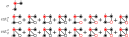
\includegraphics{extension_example}
        \caption{Example type $\sigma$ with two possible extensions}
        \label{fig:extension_example}
    \end{figure}
\end{example}

These extensions are important for the following reason:

\begin{lemma}
    If $\Gcl$ consists of only regular graphs then for any $\sigma$ and $\phi\in\Phi^\sigma$ we have
    $\phi(\ext_i^\sigma) = 1\ \forall\ i \in [|\sigma|]$.
\end{lemma}

\begin{proof}
    Let $\ext_i^\sigma=\sum_{\alpha\in I}F_\alpha$ for some index set $I$. Let
    $(G,\eta)$ be any $\sigma$-flag with $G\in\Gcl$. Then any instance of some
    $F_\alpha$ is a subset $\im\eta \subseteq U \subseteq V(G)$ where
    $G[U] \cong F_\alpha$. In particular $|U|=|F_\alpha|=|\sigma|+1=|\im\eta| + 1$ so
    $U = \im\eta \cup \{v\}$ for some $v\in V(G)$. In particular by definition of
    $\ext_i^\sigma$ this $v$ must be connected in $G$ to $\eta(i)$. Hence
    $v \in N(\eta(i))\setminus \im\eta$. This map from a copy of $F_\alpha$ in $G$ to
    a specific vertex is injective as we can
    take the $\sigma$-flag $(G[\im\eta\cup\{v\}], \eta)$ which must be isomorphic
    to $F_\alpha$. This map is also surjective for the same reason, given any
    $v\in N(\eta(i)) \setminus \im\eta$ we take $G[\im\eta \cup \{v\}$ which must
    be isomorphic to some flag $F_\alpha$ where the unlabelled vertex is connected to
    the vertex labelled $i$, so appears in the $\ext_i^\sigma$ expression.

    Therefore $\sum_{\alpha\in I}c(F_\alpha; (G,\eta)) = |N(\eta(i))\setminus\im\eta|$.
    In particular then
    \[
        \rho(\ext_i^\sigma; (G,\eta))
        = \sum_{\alpha \in I} \frac{c(F_\alpha; (G,\eta)}{\Delta(G)}
        = \frac{|N(\eta(i)) \setminus \im\eta|}{\Delta(G)}
    \]
    The size of $\im\eta$ is constant and $|N(\eta(i))|=\Delta(G)$ so this is
    in the range $[1-\frac{|\im\eta|}{\Delta(G)}, 1]$. Hence
    $\rho(\ext^\sigma_i; (G,\eta)) = 1 - o(1)$ so we do get that
    $\phi(\ext_i^\sigma)=1\ \forall\ \phi\in\Phi^\sigma$.
\end{proof}

\begin{note}
    This proof only really required that sequences of graphs in $\Gcl$ are
    \textit{asymptotically} regular so the conditions for this lemma could be relaxed
    slightly.
\end{note}

\begin{corollary}
    For any type $\sigma$ and $\phi\in\Phi^\sigma$ we
    have $\phi(\ext_i^\sigma - \ext_j^\sigma) = 0$ for all $i,j \in [|\sigma|]$
    and $\phi(f \cdot \ext_i^\sigma) = \phi(f)$ for all
    $f \in \Lcl^\sigma, i \in [|\sigma|]$.

    In particular $\ext_i^\sigma - \ext_j^\sigma\in\SemCone$,
    $f\cdot \ext_i^\sigma - f$ and $f - f\cdot\ext_i^\sigma$ are all
    elements of the semantic cone $\SemCone^\sigma$.
\end{corollary}

\begin{corollary}
    \label{corollary:unlabel_extension}
    If $\sigma$ is a local type then for any $\phi\in\Phi^\emptyset$ we have
    $\phi(\llbracket \ext_i^\sigma - \ext_j^\sigma\rrbracket) = 0$
    for all $i,j\in [|\sigma|]$ and
    $\phi(\llbracket f \cdot \ext_i^\sigma\rrbracket) = \phi(\llbracket f \rrbracket)$
    for all $f\in\Lcl^\sigma$ and $i\in [|\sigma|]$.
\end{corollary}

\begin{proof}[Proof of Corollary \ref{corollary:unlabel_extension}]
    By the previous corollary $\ext_i^\sigma - \ext_j^\sigma$ are in the
    semantic cone $\SemCone^\sigma$ so by lemma \ref{lemma:local_pos_preserve}
    we must have $\llbracket \ext_i^\sigma - \ext_j^\sigma \rrbracket \in \SemCone^\sigma$
    so $\phi(\llbracket \ext_i^\sigma - \ext_j^\sigma\rrbracket) \geq 0$.
    The same goes for swapping $i$ and $j$ so
    $\phi(\llbracket \ext_j^\sigma - \ext_i^\sigma\rrbracket) \geq 0$
    implying $\phi(\llbracket \ext_i^\sigma - \ext_j^\sigma\rrbracket) = 0$.

    The same argument works for $\llbracket f\cdot\ext_i^\sigma \rrbracket$ and
    $\llbracket f\rrbracket$.
\end{proof}

\begin{note}
    These relations suggest that if we focused only on regular graph classes
    from the beginning we could have quotiented out the set of relations
    $\llbracket \ext_i^\sigma - \ext_j^\sigma\rrbracket$ from our vector space $\R\HeredG^\emptyset$
    to get a "cleaner" algebra. I have not verified that this is possible. If this is true
    it could theoretically enable us to generate smaller semidefinite programs but we would
    need an algorithmic way of reducing vectors over this subspace which prima facie is not
    a straightforward task.
\end{note}

The value of these results for us is twofold. Firstly this gives us a wide set of
easy to generate elements of the semantic cone which we can use in our semidefinite
program. Secondly though this property where
$\phi(\llbracket f \rrbracket)=\phi(\llbracket f \cdot \ext_i^\sigma\rrbracket)$ gives
us a way of expressing a vector in a subspace of larger flags. In particular multiplying by
$\ext_i^\sigma$ gives a vector over flags which are 1 larger than those in the original
vector. This will be very useful to us.

\section{Counting Pentagons with Local Flags}

We want to use local flags to show an asymptotic bound that for any regular, triangle free
graph $G$ we have at most
$\frac{\Delta(G)^4}{8}$ 5-cycles containing any fixed $v \in V(G)$.

We first reduce this to a problem on coloured graphs.

\subsection{Reduction}

Let $G$ be a simple regular triangle free graph and fix some $v\in V(G)$. Then
$|N(v)| = \Delta(G)$ and the set $N(v)$ is independent.

First we note that as $G$ is triangle free any pentagons in $G$ are induced. Hence it
suffices to count induced pentagons only.

Any pentagon containing $v$ then must contain 2 vertices of $N(v)$ and 2 vertices
outside of $N(v)$. In particular if we construct a 3-vertex-coloured graph $H$
which is a copy of $G$ where $v$ is green, $N(v)$ is black and all others are
red then we want to count how many pentagons contain 1 green vertex, 2 black vertices
and 2 red vertices. Then as all black vertices are connected to the green vertex it
suffices to count how many black-red-red-black paths there are in $H$. In fact
removing $v$ from $H$ has no effect on this count so WLOG we can remove it.

\begin{figure}[!ht]
    \centering
    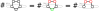
\includegraphics[scale=1.5]{pentagon_reduction}
\end{figure}

Let $\Gcl$ be the class of red-black vertex coloured graph which are triangle free,
regular, have $\Delta(G)$ black vertices and such that the set of black vertices is independent.
We want to find then an asymptotic bound on how many black-red-red-black paths we can have?
This is a problem that local flags can solve.

\subsection{Local Flags Setup}

We have decided on a class of graphs $\Gcl$ so we need to now find a description of
the local $\sigma$-flags.

\begin{lemma}
    \label{lemma:pentagon_local_flags}
    A $\sigma$-flag $F$ is a local $\sigma$-flag (relative to our choice of
    $\Gcl$) iff each connected component of $F$ contains a labelled vertex or a
    black vertex.
\end{lemma}

\begin{proof}
    First we show if each connected component of $F$ contains a labelled or black
    vertex then $F$ has bounded density function. We do this by induction on $|F|-|\sigma|$.
    The base case is that $|F|=|\sigma|$ which implies $F$ consists only of labelled
    vertices meaning $c(F; G) = 1 \in O(\Delta(G)^0)$ for any $G\in\Gcl^\sigma$
    as required.

    Otherwise assume $|F|>|\sigma|$. Note then that as each connected component of
    $F$ contains at least one labelled or black vertex each vertex $u$ of $F$ has a
    finite minimum distance $d(u)$ to some labelled or black vertex (where
    $d(u)=0$ for all black and labelled $u$ and $d(u) > 0$ for all red vertices).
    Let $v$ be some unlabelled vertex in $F$ with maximum $d(v)$. Consider then removing $v$ from
    $F$: $F' := F[V(F)\setminus \{v\}]$. This $F'$ must not have any connected
    components with no black or labelled vertices because we chose $d(v)$ large as
    possible. Hence $c(F'; G) \in O\left(\Delta(G)^{|F|-|\sigma|-1}\right)$ by our
    induction hypothesis.

    Consider then some subset $\im\eta\subseteq U' \subseteq V(G)$ such that
    $G[U'] \cong F'$. We want to bound how many copies $U$ of $F$ can we obtain
    by adding one more vertex $u\in V(G)$ onto which our removed $v$ can be mapped.
    There are 2 cases: If the $v\in V(F)$ we removed was a black vertex then
    $u$ must be a black vertex, there are only $\Delta(G)$ of those meaning there
    are $\leq \Delta(G)$ possible such $U$'s. Otherwise $v$ was a red vertex
    meaning it was connected to $V(F)\setminus\{v\}$. This means $u$ must be
    in the neighbourhood of one of the vertices of $U$ of which there are
    $O(\Delta(G))$ such options. In either case there are only $O(\Delta(G))$ such
    extensions of $U'$.
    In particular though every copy $U$ of $F$ can be reached in this way. This is easily
    seen by taking any such copy and removing the vertex $u$ that $v$ is mapped to, this must
    give you a copy $U'$ of $F'$ with which we can re-add $u$ to get back to $U$.
    Therefore this process counts all copies $U$ of $F$ in $G$ giving us a bound of
    $c(F'; G) \cdot O(\Delta(G)) = O\left(\Delta(G)^{|F|-|\sigma|}\right)$ as required.

    Now that we know any such $F$ has bounded density function we simply note that
    any label extension of $F$ gives you a new flag which also has a labelled or
    black vertex in each connected component. Therefore label extension preserves
    bounded density functions so $F$ is a local $\sigma$-flag.

    We also show that this encapsulates all local $\sigma$-flags. This isn't strictly
    required for our application so I give a brief idea of the proof. Taking any
    flag with a connected component consisting of all unlabelled red vertices we can
    easily construct a sequence of graphs $(G_k)_{k\in\N}$ in $\Gcl$ where we keep
    increasing the number of copies of the unlabelled red component. We can do this maintaining
    the fact that each $G_k$ is regular and has only $\Delta(G)$ black vertices. Then
    the number of copies of $F$ increases unbounded along this sequence proving $F$ is not
    local.
\end{proof}

Now that we know our set of local flags, which tells us our local types by
lemma \ref{lemma:local_type_equiv} we can now formulate our problem as a semidefinite
problem.

\section{The Semidefinite Program}

We fixed our class of graphs $\Gcl$ to be the class of red-black vertex coloured
regular triangle-free graphs with $\Delta(G)$ black vertices such that the set of
black vertices is independent.
We want to asymptotically bound the number of black-red-red-black paths in this
class. This means we have the following objective function: $\brrb$.
This is a local flag by lemma \ref{lemma:pentagon_local_flags}. We will now use
the semidefinite method (Section \ref{sec:semidefinite_method}) to find a bound
$\lambda\in\R$ such that $\phi(\brrb)\leq \lambda\ \forall\ \phi\in\Phi^\sigma$.

For practical purposes we want to use the subspace of $\Lcl^\emptyset$ of flags
of size 5. For this reason we find a vector $f$ over flags of size 5 such that
bounding $\phi(f)$ gives a bound on $\phi(\brrb)$. To achieve this we view
$\brrb$ as a $\brrb$-flag in itself: $\brrbmarked$.
Letting $\sigma=\brrb$ we note that $\sigma$ is a local type and we can compute
$\llbracket \brrbmarked \rrbracket=\frac{2}{4!}\brrb = \frac{1}{12}\brrb$.
We can then compute $\ext_1^\sigma$ and then use corollary \ref{corollary:unlabel_extension}
which tells us that
\[
    \frac{1}{12}\phi(\brrb) = \phi(\llbracket \brrbmarked \rrbracket)
    = \phi(\llbracket \brrbmarked \cdot \ext_1^\sigma\rrbracket).
    = \phi(\llbracket \ext_1^\sigma\rrbracket).
\]
where we used that $\sigma$ is the unit of the algebra $\Lcl^\sigma$. Then
$\ext_1^\sigma$ is a vector of flags of size 5: See figure \ref{fig:pentagon_objective}.
It suffices then to try to maximise $\llbracket \ext_1^\sigma\rrbracket$: Call this
vector $O$.

\begin{figure}[ht]
    \centering
    \includegraphics{pentagon_objective}
    \caption{$\ext^\sigma_1$ where $\sigma=\brrb$}
    \label{fig:pentagon_objective}
\end{figure}

To apply our semidefinite method we first need a list of known elements of the
semantic cone $\SemCone^\emptyset$ or dually a list of linear constraints on limit functionals.
For any type $\sigma$ we immediately get the elements
$\llbracket \ext^\sigma_i - \ext_j^\sigma\rrbracket$ from corollary
\ref{corollary:unlabel_extension}. We want only those that are in the subspace of
flags of size 5 so we take all such vectors where $|\sigma|=4$.

We know that in any $G\in\Gcl$ the set of black vertices is independent and has size
$\Delta(G)$. Let $B_k$ be the $\emptyset$-flag consisting of $k$ independent black
vertices. e.g. $B_1=\vertex, B_2=\nonedge$. Then we know $c(B_k; G) = \binom{\Delta(G)}{k}$
for any $G\in\Gcl$ which implies $\phi(B_k)=1\ \forall\ \phi\in\Phi^\emptyset\ \forall\ k\in\N$.
We would like to add these to the list of constraints. For $k=5$ this is already in
the subspace of flags of size 5 so we can add it directly. For $k < 5$ we need
to do the same extension trick as with our objective function where we use that
$\llbracket B_k \rrbracket = B_k$ to get
\[
    1 = \phi(B_k)=\phi(\llbracket B_k \rrbracket)
    = \phi(\llbracket B_k \cdot \ext_1^{B_k}\rrbracket)
    = \phi\left(\left\llbracket B_k \cdot \left(\ext_1^{B_k}\right)^{5-k}\right\rrbracket\right)
    = \phi\left(\left\llbracket \left(\ext_1^{B_k}\right)^{5-k}\right\rrbracket\right).
\]
$\left(\ext_1^{B_k}\right)^{5-k}$ is an expression over flags of size 5 so this is
a constraint we can use.

Finally then we want to encode constraints of the form $\phi(\llbracket f^2 \rrbracket) \geq 0$
for all $f\in \Lcl^\sigma$. To do this we need to find local types $\sigma$ and sizes $n$
such that $f^2$ is an expression of flags of size 5 for all $f\in\Glocn^\sigma$.
Those pairs $(\sigma, n)$ are ($\vertex$, $3$), ($\triangleempty$, $4$), ($\pentsqtypeone$, $4$),
($\pentsqtypetwo$, $4$), ($\pentsqtypethree$, $4$), and ($\pentsqtypefour$, $4$).

Let $\Bcl=(F_1, \dots, F_\ell)$ be the basis of all flags of size 5.
In summary then the dual of our SDP is:
\begin{align*}
    \max_{x\in\R^\ell}\ \ &\ \phi_x(O)\\
    \text{such that}\ \ &\ \phi_x(F_i) \geq 0\ \forall\ i \in [\ell]\\
    &\ \phi_x(\llbracket \ext^\sigma_i - \ext^\sigma_j\rrbracket) = 0\ \forall\
    |\sigma|=4, i, j \in [4]\\
    &\ \phi_x(B_5) = 1\\
    &\ \phi_x\left(\left\rrbracket\left(\ext_1^{B_k}\right)^{5-k}\right\rrbracket\right) = 1\
    \forall\ k \in [4]\\
    &\ \phi_x(\llbracket f^2 \rrbracket) \geq 0 \forall f \in \Glocn^\sigma\ \forall (\sigma, n)
    \ \text{from above list}.
\end{align*}

We know from section \ref{sec:semidefinite_method} how to construct the corresponding
SDP problem which finds a convex combination of elements of the semantic cone which solves
this problem.

Solving this SDP problem gives the upper bound of $\frac{1}{4}$ meaning
$\phi(O) \leq \frac{1}{4}\ \forall\ \phi\in\Phi^\sigma$.
We know that $\frac{1}{12}\phi(\brrb)=\phi(O)$ so $\phi(\brrb) \leq 3$.
Therefore for any $\Delta$-increasing sequence of graphs $(G_k)_{k\in\N}$ we have
$\lim_{k\to\infty} \frac{c(\brrb; G_k)}{\binom{\Delta(G_k)}{4}} \leq 3$.
Intuitively then $\binom{\Delta(G_k)}{4}$ is asymptotically $\frac{\Delta(G_k)^4}{4!}$ so
we get $\lim_{k\to\infty} c(\brrb; G_k) \leq \frac{3}{4!} = \frac{1}{8}$.
We show this argument more precisely now:

We use the fact that
$\frac{\Delta(G_k)!}{(\Delta(G_k)-4)!} = \Delta(G_k)^4 + o(\Delta(G_k)^4)$
to show that
\[
    \begin{split}
        \lim_{k\to\infty}\frac{c(\brrb; G_k)}{\Delta(G_k)^4}
        &= \lim_{k\to\infty}\frac{c(\brrb; G_k)}{\binom{\Delta(G_k)}{4}}
        \frac{\Delta(G_k)!}{4!(\Delta(G_k)-4)!\Delta(G_k)^4}\\
        &= \lim_{k\to\infty}\frac{c(\brrb; G_k)}{\binom{\Delta(G_k)}{4}}
        \frac{\Delta(G_k)^4 + o(\Delta(G_k)^4}{4!\Delta(G_k)^4}\\
        &= \lim_{k\to\infty}(1+o(1))\frac{c(\brrb; G_k)}{\binom{\Delta(G_k)}{4}}\\
        &\leq \frac{1}{8}.
    \end{split}
\]


\chapter{Application: Strong Edge Colouring}
\label{chap:strong_edge_colouring}

As defined in the \hyperref[sec:intro_strong_edge_coloring]{introduction}
a strong edge colouring of a graph is an edge colouring where two edges which are incident to some
common edge must have different colours. The minimum colours required for a strong edge colouring of
$G$ is called the strong chromatic index $\chi'_s(Gj$.
In 1985 Erd\H{o}s and Nešetřil conjectured that
$\chi'_s(G) \leq 1.73\Delta(G)^2$, and in 1989 Faudree et al. conjectured that
$\chi'_s(G) \leq \Delta(G)^2$ if $G$ is bipartite \cite{faudreeInducedMatchingsBipartite1989}.

In this chapter we will use the semidefinite method on local flags to prove the following
theorems:
\begin{knowntheorem}
    For $\Delta(G)$ large enough we have
    \[\chi'_s(G) \leq 1.73\Delta(G)^2.\]
\end{knowntheorem}
\begin{knowntheorem}
    If $G$ is bipartite then for $\Delta(G)$ large enough we have
    \[\chi'_s(G) \leq 1.6254\Delta(G)^2.\]
\end{knowntheorem}
Both of these theorems are the best known bounds in their respective cases. We start
by showing the first result, and leave the bipartite case until section
\ref{sec:sec_bipartite}.

\section{Line Graph Equivalence}

We can view a strong edge colouring of a graph as a proper vertex colour of $L(G)^2$, the
square of the line graph of $G$ (see \cite{molloyBoundStrongChromatic1997}).
The line graph $L(G)$ is a graph with a vertex $v_e$ for
each $e\in E(G)$ such that $\{v_e, v_f\} \in E(L(G))$ iff $e$ is incident to $f$ in
$G$. The square of a graph $G^2$ then is a copy of the graph where vertices at distance $\leq 2$
are connected. See figure \ref{fig:lg_example} for an example construction.

\begin{figure}[ht]
    \centering
    \includegraphics{LG_example}
    \caption{Example $G$, $L(G)$ and $L(G)^2$}
    \label{fig:lg_example}
\end{figure}

\begin{definition}[Strong Neighbourhood]
    Given a graph $G$ and edge $E \in E(G)$ define the strong neighbourhood
    $N_s(e)$ of $e$ as those edges $f \in E(G)$ which are adjacent to $e$ in 
    $L(G)^2$ (i.e. those which cannot share a colour with $e$ in a strong edge colouring).
\end{definition}

\section{The Erd\H{o}s and Nešetřil conjecture}

In 1985 Erd\H{o}s and Nešetřil \cite{faudreeInducedMatchingsBipartite1989} conjectured an
upper bound on the strong chromatic index $\chi'_s(G)$, the minimum colours needed for
a strong edge colouring.

\begin{conjecture}[Erd\H{o}s, Nešetřil 1985 \cite{faudreeInducedMatchingsBipartite1989}]
    $\chi'_s(G) \leq 1.25\Delta(G)^2$ for all graphs $G$.
\end{conjecture}

The bound of $2\Delta(G)^2$ was the best known bound until 1997 when Molloy and Reed
showed the following.
\begin{knowntheorem}[Molloy, Reed 1997 \cite{molloyBoundStrongChromatic1997}]
    $\chi'_s(G) \leq 1.998\Delta(G)^2$ for $\Delta(G)$ sufficiently large.
\end{knowntheorem}

Their proof consisted of colouring $L(G)^2$ with 2 discrete steps:
The first is a bound on the edge density of any neighbourhood of $L(G)^2$. We call
this the \textit{strong neighbourhood density}.
\begin{knownlemma}[Lemma 1 from \cite{molloyBoundStrongChromatic1997}]
    If $G$ has maximum degree $\Delta$ then for each $e\in E(G)$
    $|N_s(e)| \leq (1-\frac{1}{36})\binom{2\Delta^2}{2}$.
\end{knownlemma}
After showing the strong neighbourhoods in $L(G)^2$ are sparse they use a colouring
lemma to colour $L(G)^2$:
\begin{knownlemma}[Lemma 2 from \cite{molloyBoundStrongChromatic1997}]
    Let $\delta, \gamma > 0$ satisfy some condition. Then if
    $\Delta(H) \leq X$ such that $N(v)$ has at most $(1-\delta)\binom{X}{2}$ edges
    then $\chi(H)\leq (1-\gamma)X$.
\end{knownlemma}

This strategy of bounding the edge density of strong neighbourhoods of $G$ and
using a probabilistic colouring was iterated on through successive papers:
Bruhn and Joos found an asymptotically tight bound on the strong neighbourhood density
and improved the colouring lemma.
\begin{knowntheorem}[Bruhn \& Joos, 2015 \cite{bruhnStrongerBoundStrong2018}]
    $\chi'_s(G) \leq 1.93\Delta(G)^2$ for $\Delta(G)$ sufficiently large.
\end{knowntheorem}
Bonamy, Perett and Postle introduced a modification of the method where rather than
bounding the strong edge neighbourhood density for the entire graph we instead focus
on a subgraph of $L(G)^2$ of high degree vertices. They show that the
neighbourhood density in this subgraph can go below the tight bound of Bruhn and Joos
and so can be coloured with fewer colours. The rest of the graph has low degree so can
be coloured greedily.

\begin{knowntheorem}[Bonamy, Perrett \& Postle, 2018 \cite{bonamyColouringGraphsSparse2018}]
    If $\Delta(G)$ is sufficiently large then
    $\chi'_s(G) \leq 1.835\Delta(G)^2$.
\end{knowntheorem}

Most recently then Hurley, de Verclos and Kang improved on the colouring lemma from the
Bonamy et al. paper to achieve the current lowest known bound.
\begin{knowntheorem}[Hurley, de Verclos \& Kang, 2022 \cite{hurleyImprovedProcedureColouring2022}]
    If $\Delta(G)$ is sufficiently large then
    $\chi'_s(G) \leq 1.772\Delta(G)^2$.
\end{knowntheorem}

In this chapter we use the semidefinite method on local flags to improve the strong
neighbourhood density bound, then applying the colouring lemma from Hurley et al. as a black
box we claim the following result.

\begin{theorem}
    \label{thm:strong_edge_colouring_bound}
    If $\Delta(G)$ is sufficiently large then $\chi'_s(G) \leq 1.73\Delta(G)^2$.
\end{theorem}

The rest of this chapter is the proof of this theorem.
We will follow the same structure as used in chapter \ref{chap:pentagon_conjecture},
first reducing the problem to a problem on a certain class of coloured graphs,
finding a vector $O$ of local flags for which an asymptotic bound on the density of $O$ will allow
us to derive an asymptotic bound on the size of $|E(H[N_{H[F]}(f)])|$.
We then enumerate some elements
of the semantic cone and apply the semidefinite method to get a bound on $O$.

\section{Reduction}
\label{sec:sec_reduction}

The theorem that we want to improve on is the strong edge neighbourhood theorem from
the Bonamy et al. paper which appears in Hurley et al. as follows:
\begin{knowntheorem}[Theorem 3.1 \cite{hurleyImprovedProcedureColouring2022}]
    Fix $\eta \in [0, 0.3]$. For any graph $G$ let $H=L(G)^2$. Let $F$ be a
    maximal subset of $V(H)$ such that $H[F]$ has minimum degree
    $\geq (2-\eta)\Delta(G)^2$. Then for any $f\in F$ the number of edges in the subgraph
    $H[N_{H[F]}(f)]$ induced by the neighbourhood of $f$ (in $H[F]$) is at most
    \[
        \left(\frac{31}{6} - \frac{128}{10-3\eta} - \eta^2\right)\Delta(G)^4.
    \]
\end{knowntheorem}

In other words we are given a graph $G$ and a maximal subset of the edges $F \subseteq E(G)$
such that the subgraph induced by $F$ in $H=L(G)^2$ has minimum degree
$\geq (2-\eta)\Delta(G)^2$ for some $\eta$. This means each $f \in F$ has
at least $(2-\eta)\Delta(G)^2$ other edges $f' \in F$ adjacent in $L(G)^2$
($|N_s(f) \cap F| \geq (2-\eta)\Delta(G)^2\ \forall\ f \in F$).
We can then just consider the graph $H[F]$ induced by this high degree $F$ subset.
Then for some fixed $f \in F$ we want to find an upper bound on the number of edges
in its neighbourhood in $H[F]$. That is, the number of pairs $e, e' \in N_s(f) \cap F$ such
that $e, e'$ adjacent in $L(G)^2$.

\begin{note}
    The first reduction we can note is that WLOG we can assume $G$ is regular,
    as outlined in each of the above papers.
\end{note}

We note now that asymptotically it suffices to count only the number of edges
in $H[N_{H[F]}(f)]$ which correspond to pairs $e, e'\in E(G)$ which are not incident.
i.e. those $e,e'$ which are adjacent in $L(G)^2$ but not $L(G)$.
\begin{lemma}
    \label{lemma:count_non_incident_pairs}
    Let $G, F, H$ and $f\in F$ be as above. Let $A$ be those pairs $e,e'\in F$
    such that $e, e'$ adjacent in $L(G)^2$ but not $L(G)$.
    Then
    \[
        |E(H[N_{H[F]}(f)])| = |E(H[N_{H[F]}(f)]) \cap A| + o(\Delta(G)^4).
    \]
\end{lemma}
\begin{proof}
    We count how many pairs $e, e' \in N_s(f) \cap F$ are adjacent in $L(G)$.
    Clearly $|N_s(f)| \in O(\Delta(G)^2)$ and each $e \in N_s(f)$ has $O(\Delta)$
    incident edges leading to a bound of $O(\Delta(G)^3) \subseteq o(\Delta(G)^4)$
    as required.
\end{proof}

Similarly, the condition that $\deg_{H[F]}(f) \geq (2-\eta)\Delta(G)^2$ for all
$f\in F$ is dominated only by non-incident edges.
\begin{lemma}
    \label{lemma:sec_degree_non_incident}
    Let $G, F, H$ and $f\in E(G)$ be as above. Let $B$ be those edges $e\in F$
    such that $e$ is adjacent to $f$ in $L(G)^2$ but not in $L(G)$.
    Then
    \[
        \deg_{H[F]}(f) = |B| + o(\Delta(G)^2).
    \]
\end{lemma}
\begin{proof}
    The number of edges incident to a fixed $f$ in $L(G)$ is $O(\Delta(G))$.
\end{proof}

As we did in section \ref{sec:counting_pentagons} we want to reduce our problem to a
problem on coloured graphs.
Given $G$, $F\subseteq E(G)$, $\eta > 0$ and $f \in F$ as above we can construct a
new corresponding $(2,2)$-graph (red/black vertices, red/black edges) $G'$ as follows:
Let $f=\{u, v\}$. Take a copy of $G$ and colour all neighbours of $u$ and $v$ black
and all other vertices red. Then colour every edge $e \in F$ black and all other
edges red. See figure \ref{fig:transform} for example.

\begin{figure}[ht]
    \centering
    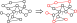
\includegraphics[scale=1]{sec_transform}
    \caption{Example coloured graph transformation}
    \label{fig:transform}
\end{figure}

\begin{lemma}
    \label{lemma:sec_black_edge_degree}
    Let $G, H=L(G)^2, F, \eta, f$ and $G'$ be as above.
    Define $E_O(G') \subseteq \binom{E(G')}{2}$ as the set of pairs of non-incident
    edges $e, e'$ in $G'$
    where $e, e'$ are black edges with a common incident edge and
    at least one of the vertices of each edge is black.
    Then the number of edges in $H[N_{H[F]}(f)]$
    where $H=L(G)^2$ is equal to $|E_O(G')| + o(\Delta(G)^4)$.
\end{lemma}

\begin{proof}
    Let $G$, $H=L(G)^2$, $F, \eta, f$ and $G'$ be as above.
    By lemma \ref{lemma:count_non_incident_pairs} it suffices to show the result for
    number of pairs $e,e'$ in $H[N_{H[F]}(f)]$ where $e,e'$ are not incident.

    Consider some edge $\{e, e'\}$ in
    $H[N_{H[F]}(f)]$ where $e,e'$ are not incident.
    Both of these $e,e'$ are in $F$ so are coloured black in $G'$.
    Similarly both are in the strong neighbourhood of $f$ meaning each has a common
    incident edge with $f$. Edges incident to $f$ have both vertices coloured black
    in $G'$ so each of $e, e'$ has at least one black vertex.
    Hence this edge $\{e, e'\}$ corresponds to a pair of non-incident black edges with at least one
    black vertex each in $G'$ at distance $\leq 2$ from each other.

    Consider then some pair $e,e' \in E_O(G')$
    As each $e,e'$ has a black vertex they must be either incident to $f$ \textit{or} equal
    to $f$. If both $e, e' \neq f$ then
    $e, e'$ satisfy exactly the conditions to be an edge in $H[N_{H[F]}(f)]$.
    Hence we overcount the number of edges in $H[N_{H[F]}(f)]$ by exactly the
    number of these pairs $e, e'\in E_0$ where one of $e, e' = f$. Assume $e=f$,
    this leaves only $\leq 2\Delta(G)^2$ choices for $e'$ so there are at most
    $2\Delta(G)^2$ such pairs which is $o(\Delta(G)^4)$ as required.
\end{proof}

\begin{corollary}
    \label{corollary:strong_density_graph_class}
    It suffices to bound the size of $E_O$
    over the class of all regular $(2,2)$-graphs where there are $\leq 2\Delta(G)^2$ black
    vertices and the subgraph of $L(G)^2$ induced by black edges has minimum
    degree $\geq (2-\eta)\Delta(G)^2$.
\end{corollary}

This is something we can bound with local flags.

\section{Local Flag Setup}

Let $\Gcl$ be the class of graphs described in corollary \ref{corollary:strong_density_graph_class}.
As before the hereditary closure $\HeredG$ only drops the regularity requirement.

\begin{lemma}
    Given the class $\Gcl$ and $\Delta$ as the max-degree function then a
    $\sigma$-flag $(F, \theta)\in \HeredG{}^\sigma$ is a local-$\sigma$ flag (definition
    \ref{def:local_flag}) iff
    each connected component of $F$ contains at least one black vertex or labelled vertex.
\end{lemma}

\begin{proof}
    See proof of lemma \ref{lemma:pentagon_local_flags}.
\end{proof}

\subsection{Objective Vector}
\label{sec:sec_obj_vector}

First we want to express the size of $E_O(G)$ as a local flag vector.
Note if $\Bcl\subseteq G$ is the set of black edges with at least one black vertex then
\[
    2|E_O(G)| = \sum_{e \in \Bcl}|\{e' \in \Bcl \colon e, e'\ \text{have common edge}\}|
\]
We can split $\Bcl$ further into $\Bcl_1$ and $\Bcl_2$, the set of edges with one
black and one red vertex and the set of edges with two black vertices respectively.
\begin{multline*}
    2|E_O(G)| = \sum_{e \in \Bcl_1}|\{e' \in \Bcl \colon e, e'\ \text{have common edge}\}|\\
    +  \sum_{e \in \Bcl_2}|\{e' \in \Bcl \colon e, e'\ \text{have common edge}\}|
\end{multline*}

The $\sigma_1=\bredge$ is a local type by lemma \ref{lemma:local_type_equiv}. Clearly
for any $e\in \Bcl_1$ we can view $G$ as a $\sigma_1$-flag where $\sigma_1$ is mapped
to $e$. Call this $G^e$. Similarly any $\sigma_1$-embedding corresponds to precisely one
$e\in \Bcl_1$.
Fix some $e\in \Bcl_1$, then take some $e'\in\Bcl$ such that $e,e'$ have a common incident edge.
Then the vertices of $e,e'$ in $G^e$ induce some subgraph of size 4 where the two unlabelled
vertices (those corresponding to $e'$) have a black edge and there is a single connected
component. Conversely any such induced subgraph corresponds to exactly one $e' \in \Bcl$.
Hence we can count such $e'$'s there are by counting how many such induced subgraphs
there are. These subgraphs are easily enumerated.

Define $D(\bredge) \in \Lcl^{\sigma_1}$ to be the vector consisting of the sum of all
local $\sigma_1$-flags of size 4 with a black edge between the unlabelled vertices and a
single connected component:
\[
    \begin{split}
        D(\bredge) &:= 
        \secdbr{5in4t2id2} + \secdbr{6in4t2id2} + \secdbr{7in4t2id2} + \secdbr{13in4t2id2} + \secdbr{14in4t2id2} + \secdbr{15in4t2id2} + \secdbr{21in4t2id2} + \secdbr{22in4t2id2} + \secdbr{23in4t2id2}\\
		& \secdbr{29in4t2id2} + \secdbr{30in4t2id2} + \secdbr{31in4t2id2} + \secdbr{37in4t2id2} + \secdbr{38in4t2id2} + \secdbr{39in4t2id2} + \secdbr{45in4t2id2} + \secdbr{46in4t2id2} + \secdbr{47in4t2id2}\\
		& \secdbr{53in4t2id2} + \secdbr{54in4t2id2} + \secdbr{55in4t2id2} + \secdbr{61in4t2id2} + \secdbr{62in4t2id2} + \secdbr{63in4t2id2} + \secdbr{74in4t2id2} + \secdbr{75in4t2id2} + \secdbr{84in4t2id2}\\
		& \secdbr{85in4t2id2} + \secdbr{86in4t2id2} + \secdbr{96in4t2id2} + \secdbr{97in4t2id2} + \secdbr{98in4t2id2} + \secdbr{108in4t2id2} + \secdbr{109in4t2id2} + \secdbr{110in4t2id2} + \secdbr{120in4t2id2}\\
		& \secdbr{121in4t2id2} + \secdbr{122in4t2id2} + \secdbr{132in4t2id2} + \secdbr{133in4t2id2} + \secdbr{134in4t2id2} + \secdbr{144in4t2id2} + \secdbr{145in4t2id2} + \secdbr{146in4t2id2} + \secdbr{156in4t2id2}\\
		& \secdbr{157in4t2id2} + \secdbr{158in4t2id2} + \secdbr{169in4t2id2} + \secdbr{170in4t2id2} + \secdbr{179in4t2id2} + \secdbr{180in4t2id2} + \secdbr{181in4t2id2} + \secdbr{191in4t2id2} + \secdbr{192in4t2id2}\\
		& \secdbr{193in4t2id2} + \secdbr{203in4t2id2} + \secdbr{204in4t2id2} + \secdbr{205in4t2id2} + \secdbr{215in4t2id2} + \secdbr{216in4t2id2} + \secdbr{217in4t2id2} + \secdbr{227in4t2id2} + \secdbr{228in4t2id2}\\
		& \secdbr{229in4t2id2} + \secdbr{239in4t2id2} + \secdbr{240in4t2id2} + \secdbr{241in4t2id2} + \secdbr{252in4t2id2} + \secdbr{253in4t2id2} + \secdbr{262in4t2id2} + \secdbr{263in4t2id2} + \secdbr{264in4t2id2}\\
		& \secdbr{274in4t2id2} + \secdbr{275in4t2id2} + \secdbr{276in4t2id2} + \secdbr{286in4t2id2} + \secdbr{287in4t2id2} + \secdbr{288in4t2id2} + \secdbr{298in4t2id2} + \secdbr{299in4t2id2} + \secdbr{300in4t2id2}\\
		& \secdbr{310in4t2id2} + \secdbr{311in4t2id2} + \secdbr{312in4t2id2} + \secdbr{323in4t2id2} + \secdbr{324in4t2id2} + \secdbr{333in4t2id2} + \secdbr{334in4t2id2} + \secdbr{335in4t2id2} + \secdbr{345in4t2id2}\\
		& \secdbr{346in4t2id2} + \secdbr{347in4t2id2} + \secdbr{357in4t2id2} + \secdbr{358in4t2id2} + \secdbr{359in4t2id2} + \secdbr{369in4t2id2} + \secdbr{370in4t2id2} + \secdbr{371in4t2id2} + \secdbr{382in4t2id2}\\
		& \secdbr{383in4t2id2} + \secdbr{392in4t2id2} + \secdbr{393in4t2id2} + \secdbr{394in4t2id2} + \secdbr{404in4t2id2} + \secdbr{405in4t2id2} + \secdbr{406in4t2id2} + \secdbr{416in4t2id2} + \secdbr{417in4t2id2}\\
		& \secdbr{418in4t2id2} + \secdbr{429in4t2id2} + \secdbr{430in4t2id2} + \secdbr{439in4t2id2} + \secdbr{440in4t2id2} + \secdbr{441in4t2id2} + \secdbr{451in4t2id2} + \secdbr{452in4t2id2} + \secdbr{453in4t2id2}\\
		& \secdbr{464in4t2id2} + \secdbr{465in4t2id2} + \secdbr{474in4t2id2} + \secdbr{475in4t2id2} + \secdbr{476in4t2id2} + \secdbr{487in4t2id2} + \secdbr{488in4t2id2}
    \end{split}
\]
Then by the above $\rho(D(\bredge); G^e) = \frac{|\{e' \in \Bcl\colon e,e'\ \text{have common edge}\}}{\binom{\Delta(G)}{2}}$.

We can then use lemma \ref{lemma:local_averaging_exp} to note that
\[
    \begin{split}
        \rho(\llbracket D(\bredge) \rrbracket; G) 
        &\sim \rho(\llbracket \bredge\rrbracket; G) \E_\theta[\rho(D(\bredge), (G,\theta))]\\
        &= \frac{1}{2}\frac{\sum_{e\in\Bcl_1}|\{e' \in \Bcl\colon e,e'\ \text{have common edge}\}|}{\binom{\Delta(G)}{2}\binom{\Delta(G)}{2}}
    \end{split}
\]

We can do the exact same construction with $\sigma_2 = \edge$. The only thing we have to note is that for any $e\in \Bcl_2$ there are two ways to embed $\sigma_2$ so defining $D(\edge)$ in
the same way we get a double count of
$\rho(D(\edge); G^e) = 2\frac{|\{e' \in \Bcl\colon e,e'\ \text{have common edge}\}}{\binom{\Delta(G)}{2}}$
hence applying lemma \ref{lemma:local_averaging_exp} again we get
\[
    \begin{split}
        \rho(\llbracket D(\edge) \rrbracket; G) 
        &\sim \rho(\llbracket \edge\rrbracket; G) \E_\theta[\rho(D(\bredge), (G,\theta))]\\
        &= \frac{\sum_{e\in\Bcl_2}|\{e' \in \Bcl\colon e,e'\ \text{have common edge}\}|}{\binom{\Delta(G)}{2}\binom{\Delta(G)}{2}}
    \end{split}
\]
Therefore
\[
    \rho(2\llbracket D(\bredge)\rrbracket + \llbracket D(\edge)\rrbracket; G)
    \sim \frac{2|E_O(G)|}{\binom{\Delta(G)}{2}\binom{\Delta(G)}{2}}
\]
so we pick $2\llbracket D(\bredge)\rrbracket + \llbracket D(\edge)\rrbracket$
as the vector we want to find a density bound for.

In general when applying the semidefinite method we will want a vector
over local flags of some fixed size $n$. Luckily our class $\Gcl$ consists of regular
graphs so we can use the extension vectors from section \ref{sec:local_flags_regular_graphs}
and corollary \ref{corollary:unlabel_extension}
to get a vector equivalent to $2\llbracket D(\bredge)\rrbracket + \llbracket D(\edge)\rrbracket$.
We define then our final objective vector $O$ to be
\[
    O := 2\left\llbracket D(\bredge) \cdot \left(\ext^\bredge_1\right)^{n-4} \right\rrbracket
        + \left\llbracket D(\edge) \cdot \left(\ext^\edge_1\right)^{n-4}\right\rrbracket
\]
for some $n\geq 4$ yet to be chosen.

\begin{lemma}
    \label{lemma:sec_objective}
    \[
        \rho(O; G) \sim \frac{2|E_O(G)|}{\binom{\Delta(G)}{2}\binom{\Delta(G)}{2}}
        \ \text{as}\ \Delta(G) \to \infty
        \ \forall\ G\in\Gcl
    \]
\end{lemma}
\begin{proof}As outlined above\end{proof}

\subsection{Search Constraints}
\label{sec:sec_search_constraints}

As in chapter \ref{chap:pentagon_conjecture}, we want to collect some known elements of
the semantic cone where each vector consists of local flags of some fixed size $n$.
(Dually this corresponds with finding linear constraints on limit functionals).
As $\Gcl$ is a class of regular graphs we get the constraints of
the form $\llbracket \ext^\sigma_i - \ext^\sigma_j\rrbracket$ from corollary
\ref{corollary:unlabel_extension} as we did in section \ref{sec:pentagon_sdp}.

First we find some constraints which encode the property
that the minimum degree of the subgraph of
$L(G)^2$ induced by black edges is $\geq (2-\eta)\Delta(G)^2$. In other words
for each black edge $e$ the number of other black edges in $G$ with a common
incident edge is $\geq (2-\eta)\Delta(G)^2$. Following how we defined $D(\bredge)$ 
we define $D'(\sigma)$ for $\sigma\in\{\edge,\bredge\}$ as the sum of
local $\sigma$-flags of size 4 where the unlabelled
vertices form a black edge. Let $e\in E(G)$ be an edge of the form $\bredge$. Then
by lemma \ref{lemma:sec_degree_non_incident} we have:
\[
    \rho(D'(\bredge); G^e) = \frac{\deg_{H[F]}(e)}{\binom{\Delta(G)}{2}} - o(1)
    \geq \frac{2\deg_{H[F]}(e)}{\Delta(G)^2} - o(1)
    \geq 2(2-\eta) - o(1)
\]
Hence $\phi(D'(\bredge)) \geq 2(2-\eta)\ \forall\ \phi \in \Phi^\bredge$.
In particular then
\[
    \begin{split}
        \phi((D'(\bredge) - 2(2-\eta)(\ext_1^\bredge)^2) \cdot \left(\ext_1^\bredge\right)^{n-4}) \geq 0
        \ \forall\ \phi \in \Phi^\bredge\\
        \implies \phi\left( \left\llbracket (D'(\bredge) - 2(2-\eta)(\ext_1^\bredge)^2) \cdot
        \left(\ext_1^\bredge\right)^{n-4}\right\rrbracket\right)\geq 0
        \ \forall\ \phi \in \Phi^\emptyset\\
    \end{split}
\]
by corollary \ref{corollary:unlabel_extension} and lemma \ref{lemma:local_pos_preserve}
giving us another constraint. We could add the same constraint for $\edge$ but in practice
it suffices to only add this one.

Next we want to encode the fact that there are at most $2\Delta(G)$ black vertices.
For any type $\sigma$ we can define the
\textit{black vertex extension vector of size $k$} $\ext_{B,k}^\sigma$ as the sum of all
local flags of size $|\sigma|+k$ where the unlabelled vertices are black vertices.

\begin{lemma}
    \label{lemma:black_extension_vector}
    For a graph $G$ let $B(G)$ denote the set of black vertices
    and $i\in \N$. Consider a $\sigma$-flag $(G, \eta)$ then
    \[
        \rho(\ext_{B,i}^\sigma; (G,\eta))
        = \frac{\binom{|B(G) \setminus \im\eta|}{i}}{\binom{\Delta(G)}{i}}
        \sim 
        \left(\frac{|B(G)\setminus\im\eta|}{\Delta(G)}\right)^i
    \]
\end{lemma}
\begin{proof}
    Consider a $\sigma$-flag $(G, \eta)$.
    Given any set of black vertices $V\subseteq B(G)\im\eta$ of size $i$ we can induce a subgraph
    $\im\eta \cup V$ of size $|\sigma|+i$ which is counted by some local $\sigma$-flag
    of size $|\sigma|+i$ where the unlabelled vertices are black. Similarly every
    $U=\im\eta \cup V$ which is isomorphic to some local $\sigma$-flag where the unlabelled
    vertices are black implies $V \subseteq B(G)\setminus\im\eta$.
\end{proof}
\begin{corollary}
    For any type $\sigma$ $\phi(\ext_{B,i}^\sigma) \leq 2^i$ for all $\phi\in\Phi^\sigma$,
    $i\in\N$.
\end{corollary}
\begin{corollary}
    For any type $\sigma$, $i\in\N$ we have $\phi(\ext_{B,i}^\sigma) = \phi(\ext_{B,1}^\sigma)^i$
\end{corollary}
\begin{corollary}
    For any type $\sigma$, $i\in [|\sigma|]$ $\phi(2\ext_i^\sigma - \ext_{B,1}^\sigma) \geq 0\ \forall
    \phi\in\Phi^\sigma$.
    If $\sigma$ is a local type then
    $\phi(\llbracket 2\ext_i^\sigma - \ext_{B,1}^\sigma\rrbracket) \geq 0\ \forall\
    \phi\in\Phi^\emptyset$.
\end{corollary}

Then we can add the constraint that
\[\llbracket 2\ext_i^\sigma - \ext_{B,1}^\sigma\rrbracket \geq 0\]
for all
local types $\sigma$ of size $n-1$. Similarly for local type $\sigma=\vertex$ we can
add the constraints
\[\phi(\llbracket (\ext_{B,1}^k - \ext_{B,k}) \cdot (\ext_1^\sigma)^{n-k-1} \rrbracket) = 0\]
for all $2 \leq k \leq n-1$ which are all constraints over flags of size $n$.

We then we add the constraint using $\sigma=\vertex$ that
$\phi(\llbracket \vertex \cdot \ext_1^{n-1}\rrbracket) \leq 2$
which holds because $\llbracket O \rrbracket = O$.

Finally then we add the constraints of the form
$\phi(\llbracket f^2 \rrbracket) \geq 0$ for all $f\in\Lcl^\sigma$
for all local types $\sigma$. As we did in chapter \ref{chap:pentagon_conjecture} we pick a
subspace of $\Lcl^\sigma$ of flags of some size $m$ such that $f^2$ is a vector over
flags of size $n$ for each $f$ in the subspace. In particular this means $2m-|\sigma|=n$.

Letting $\Bcl=(F_1, \dots, F_\ell)$ be a list of local $\sigma$-flags of size $n$
we have the following optimisation problem:

\begin{align*}
    \max_{x\in\R^\ell}\ \ &\ \phi_x(O)\\
    \text{such that}\ \ &\ \phi_x(F_i) \geq 0\ \forall\ i \in [\ell]\\
    &\ \phi_x(\llbracket \ext^\sigma_i - \ext^\sigma_j\rrbracket) = 0\ \forall
    \ \text{local types}\ |\sigma|=n-1, i, j \in [n-1]\\
    &\ \phi_x\left( \left\llbracket (D'(\bredge) - 2(2-\eta)(\ext_1^\bredge)^2) \cdot
    \left(\ext_1^\bredge\right)^{n-4}\right\rrbracket\right)\geq 0\\
    &\ \phi_x(\llbracket 2\ext_1^\sigma - \ext_{B,1}^\sigma\rrbracket) \geq 0\ \forall
    \ \text{local types}\ |\sigma|=n-1\\
    &\ \phi_x(\llbracket (\ext_{B,1}^k - \ext_{B,k}) \cdot (\ext_1^\sigma)^{n-k-1} \rrbracket) = 0
    \ \text{for}\ \sigma=\vertex, \ \forall\ 2 \leq k \leq n-1\\
    &\ \phi_x(\llbracket f^2 \rrbracket) \geq 0 \forall f \in \Lcl_m^\sigma
    \ \forall\ \sigma\ \text{local type}\ \forall\ 2m-|\sigma|=n
\end{align*}

As with chapter \ref{chap:pentagon_conjecture} we know from section
\ref{sec:sdp_duality} how to convert this to a rigorous SDP which will find an
element $\lambda\emptyset - O \in \SemCone^\emptyset$.
This program however has a dependency on the parameter $\eta > 0$. For any fixed
value of $\eta$ we can find an upper bound on $\phi(O)$ but we cannot use this
approach to find a general closed form for such a bound in terms of $\eta$.
In practice though to prove theorem \ref{thm:strong_edge_colouring_bound}
we need only to find some "good" value of $\eta$. We found such an $\eta$ using
a search method described in appendix TODO.

We use our SDP software (appendix \ref{app:flag_software}) and choose $n=5$ to find the following
bound:
\begin{lemma}
    \label{lemma:sec_sdp_soln}
    For $\eta = 0.2703$ we have
    \[
        10.644\emptyset - O \in \SemCone^\emptyset
    \]
\end{lemma}

We will not translate the SDP solution back to a separate proof here as we did in
section \ref{sec:pentagon_proof_validation}, instead we leave details on verifying
the construction to appendix TODO.

Now we can prove theorem \ref{thm:strong_edge_colouring_bound}.
\begin{proof}[Proof of theorem \ref{thm:strong_edge_colouring_bound}]
    Let $\eta = 0.2703$ and $\lambda\in\R$ be such that we have a bound of
    $\phi(O) \leq \lambda\ \forall\ \phi\in\Phi^\emptyset$.
    Then by lemma \ref{lemma:sec_objective} we have
    \[
        \lim_{\Delta(G) \to \infty}
        \frac{2|E_O(G)|}{\binom{\Delta(G)}{2}\binom{\Delta(G)}{2}}
        \leq \lambda.
    \]
    This then implies that
    \[
        \lim_{\Delta(G) \to \infty}
        \frac{|E_O(G)|}{\Delta(G)^4}
        \leq \frac{\lambda}{8}.
    \]
    We use corollary \ref{corollary:strong_density_graph_class} to translate from
    coloured graphs back to simple graphs and get that for any graph $G$,
    $H = L(G)^2$, maximal subset $F\subseteq E(G)$ such that $H[F]$ has minimum degree
    $\geq (2-\eta)\Delta(G)^2$ and some $f\in F$ we have
    \[
        \lim_{\Delta(G) \to \infty}
        \frac{|E(H[N_{H[F]}(f)])| + o(\Delta(G)^4)}{\Delta(G)^4}
        \leq \frac{\lambda}{8}
        \implies
        \lim_{\Delta(G) \to \infty}
        \frac{|E(H[N_{H[F]}(f)])|}{\Delta(G)^4}
        \leq \frac{\lambda}{8}.
    \]
    In order to apply the colouring lemma from Hurley, de Verclos and Kang
    \cite{hurleyImprovedProcedureColouring2022} we need to find $\sigma\in\R$ such that
    $|E(H[N_{H[F]}(f)])| \leq (1-\sigma)\binom{2\Delta(G)^2}{2}$ for $\Delta(G)$ large
    enough. We can use the fact that
    $\binom{2\Delta(G)^2}{2} = 2\Delta(G)^4 - o(\Delta(G)^4)$
    to see that $\sigma = (1-\frac{\lambda}{16})$ suffices.

    Now we can apply Theorem 1.2 from Hurley et al \cite{hurleyImprovedProcedureColouring2022}
    which states that for any $\iota > 0$ there is some $\Delta_0$ large enough such that
    $\chi(H[F]) \leq (1-\varepsilon(\sigma) + \iota)2\Delta(G)^2$
    where $\varepsilon(\sigma) = \sigma/2 - \sigma^{3/2}/6$.

    Evaluating $\varepsilon(\sigma)$ for $\lambda = 10.644$ from 
    lemma \ref{lemma:sec_sdp_soln} gives a bound of
    $\chi(H[F]) \leq (1.72981 + \iota)\Delta(G)^2$
    Note then $2-\eta = 1.7297 < 1.73$ so by the proof of Theorem 1.6 in
    \cite{hurleyImprovedProcedureColouring2022}
    this proves $\chi(H) \leq 1.73\Delta(G)^2$ proving
    $\chi'_s(G) \leq 1.73\Delta(G)^2$ for $\Delta(G)$ large enough.
\end{proof}
\begin{note}
    A more careful validation of the dual solution from the SDP solver is required,
    but for the purposes of this thesis we considered it unnecessary as it is is not
    mathematically interesting. I give a brief discussion of how you can do this in
    appendix TODO.
    After such a validation of the floating point error you could in theory get
    a strictly below 1.73. We don't do this
    as any such result is negligibly better than 1.73 so not very interesting.
\end{note}

\section{The Bipartite Case}
\label{sec:sec_bipartite}

In 1989 Faudree, Gyárfas, Schelp and Tuza
made a conjecture that for the special case where $G$ is bipartite we get a tighter
upper bound on the strong chromatic index.

\begin{knownconjecture}[Faudree, Gyárfas, Schelp, Tuza \cite{faudreeInducedMatchingsBipartite1989}]
    If $G$ is bipartite then $\chi'_s(G) \leq \Delta(G)^2$.
\end{knownconjecture}

From what we can find, there are no papers showing a better bound than the general
bounds for the special case of bipartite graphs. Luckily for us the method of local flags
is easily specialised to the case of bipartite graphs meaning we can make the first
progress toward this conjecture. This is a big advantage of the method of local flags,
the methods used in previous papers to bound the strong neighbourhood density do not seem
to be so easily adaptable to a special case like this.

We claim the following theorem:
\begin{theorem}
    \label{thm:sec_bipartite_bound}
    If $G$ is bipartite then for $\Delta(G)$ large enough we have
    \[\chi'_s(G) \leq 1.6254\Delta(G)^2.\]
\end{theorem}

The first thing we do is adapt our reduction from section \ref{sec:sec_reduction}. Once
again we can assume WLOG that $G$ is regular. Assume we are given
$G$, $F \subseteq E(G)$, $\eta > 0$ and $f\in F$ as before except now $G$ is bipartite.

\begin{figure}[ht]
    \centering
    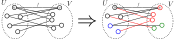
\includegraphics[scale=0.75]{bipartite_sec_transform}
    \caption{Example coloured graph transformation}
    \label{fig:bipartite_sec_transform}
\end{figure}

Once again we show how to convert $(G,F,f)$ to an equivalent coloured graph. In this case
we will use a $(4, 2)$-graph. First we pick some fixed bipartition of the vertices
of $G$, $V(G) = U \sqcup V$. This is possible as $G$ is bipartite and we can take any
such partition. Let $f=\{u,v\}$ such that $u\in U$ and $v\in V$.

Colour the neighbours of $u$ red, and the neighbours of $v$ black. Note
$N(u) \subseteq V$ and $N(v)\subseteq U$. Then colour the remaining vertices of
$U$ and $V$ blue and green respectively. Finally colour edges black if they are
$\in F$, otherwise red. See figure \ref{fig:bipartite_sec_transform} for an example.

Now, we can adopt lemmas \ref{lemma:count_non_incident_pairs} and
\ref{lemma:sec_degree_non_incident} as in the previous section.
Then we can also use the following lemma which is identical to lemma
\ref{lemma:sec_black_edge_degree}:
\begin{lemma}
    Let $G, H=L(G)^2, F, \eta, f$ and $G'$ be as above.
    Define $E_O(G') \subseteq \binom{E(G')}{2}$ as the set of pairs of non-incident
    edges $e, e'$ in $G'$
    where $e, e'$ are black edges with a common incident edge and
    at least one of the vertices of each edge is black \textbf{or red}.
    Then the number of edges in $H[N_{H[F]}(f)]$
    where $H=L(G)^2$ is equal to $|E_O(G')| + o(\Delta(G)^4)$.
\end{lemma}
\begin{proof}
    Follow the proof of lemma \ref{lemma:sec_black_edge_degree}.
\end{proof}
\begin{corollary}
    \label{corollary:bipartite_strong_density_graph_class}
    It suffices to bound the size of $E_O(G)$
    over the class $\Gcl$ of all regular $(4,2)$-graphs where there are $\Delta(G)^2$ black
    vertices, $\Delta(G)$ red vertices, the subgraph of $L(G)^2$ induced by
    black edges has minimum degree $\geq (2-\eta)\Delta(G)^2$ and the graph can be
    bi-partitioned into the components of blue/black vertices and red/green vertices.
\end{corollary}

We therefore choose our graph class $\Gcl$ as the one from
corollary \ref{corollary:bipartite_strong_density_graph_class} and as with the
previous section we get $\HeredG$ as the same class without the regularity requirement
and the following description of local flags.

\begin{lemma}
    Given the class $\Gcl$ and $\Delta$ as the maximum degree function a
    $\sigma$-flag $(F,\theta)\in\HeredG{}^\sigma$ iff each connected component
    of $F$ contains at least one black, red or labelled vertex.
\end{lemma}
\begin{proof}
    See proof of lemma \ref{lemma:pentagon_local_flags}.
\end{proof}

\subsection{Objective Vector}

As with section \ref{sec:sec_obj_vector} we'll define $D(\sigma)$ where
$\sigma \in \{\bredge,\blredge,\bgedge\}$ as the sum of all local $\sigma$-flags
of size 4 where the unlabelled vertices form a black edge which is connected
to the labelled vertices and at least one unlabelled vertex is red or black. Then we have:
\[
    \rho\left(\llbracket D(\bredge) \rrbracket
    + \llbracket D(\blredge) \rrbracket
    + \llbracket D(\bgedge) \rrbracket; G'\right)
    \sim \frac{|E_O(G)|}{\binom{\Delta(G)}{2}\binom{\Delta(G)}{2}}
\]
by the same derivation as in section \ref{sec:sec_obj_vector}. Hence we define
the objective vector $O$ as
\[
    O := \left\llbracket D(\bredge) \cdot \left(\ext^\bredge_1\right)^{n-4} \right\rrbracket
        + \left\llbracket D(\blredge) \cdot \left(\ext^\blredge_1\right)^{n-4}\right\rrbracket
        + \left\llbracket D(\bgedge) \cdot \left(\ext^\bgedge_1\right)^{n-4}\right\rrbracket
\]
for $n\in\N$ yet to be chosen and get the following result:
\begin{lemma}
    \label{lemma:sec_bipartite_objective}
    \[
        \rho(O; G) \sim \frac{|E_O(G)|}{\binom{\Delta(G)}{2}^2}.
    \]
    as $\Delta(G) \to \infty$ for all $G\in\Gcl$.
\end{lemma}
\begin{proof}
    As above.
\end{proof}

\subsection{Constraints}

Following the pattern of this thesis we now list some constraints on the space of
limit functionals and find ways to express them in the basis of flags of fixed size
$n$. As $\Gcl$ is a regular class we get the constraints of the form
$\phi(\llbracket \ext^\sigma_i \ext^\sigma_j \rrbracket) = 0$ for all local types
$\sigma$, $i,j\in[|\sigma|]$. We can add these for all local $\sigma$ of size
$n-1$.

We then define $D'(\sigma)$ as we did in section
\ref{sec:sec_search_constraints} for $\sigma\in\{\bredge,\blredge,\bgedge\}$ to be
the sum of all $\sigma$-flags of size 4 where the unlabelled vertex is a black edge
connected to the labelled vertices, then again in the same construction
find that (using lemma \ref{lemma:sec_degree_non_incident})
\[\rho(D'(\sigma); G^e) \geq 2(2-\eta)-o(1)\]
for any $G\in\Gcl$, $e\in E(G)$ of type $\sigma$. Then as we did in section
\ref{sec:sec_search_constraints} we can add the following constraints to our
list:
\[
    \phi\left(\left\llbracket
    \left(D'(\sigma) - 2(2-\eta)(\ext_1^\sigma)^2\right)\cdot \left(\ext_1^\sigma\right)^{n-4}
    \right\rrbracket\right)
    \geq 0\ \forall\ \phi\in\Phi^\emptyset
\]
for all $\sigma$ above.

Finally then we add some constraints to add the fact that there are
$\Delta(G)$ black and red vertices. As we did in section
\ref{sec:sec_search_constraints} we define the
\textit{black and red vertex extension vectors of size $k$} denoted
$\ext_{B,k}^\sigma$ and $\ext_{R,k}^\sigma$ respectively, as the sum of all
local flags of size $|\sigma|+k$ where the unlabelled vertices are black
and red respectively.
Then as with lemma \ref{lemma:black_extension_vector} we get the following result:

\begin{lemma}
    For a graph $G\in\Gcl$ let $B(G)$ and $R(G)$ denote the set of black vertices and
    $k\in \N$. Then for a $\sigma$-flag $(G,\eta) \in \Gcl^\sigma$ we have
    \[
        \begin{split}
            \rho\left(\ext_{B,i}^\sigma; (G,\eta)\right)
            &= \frac{\binom{|B(G) \setminus \im\eta|}{i}}{\binom{\Delta(G)}{i}}
            \sim 
            \left(\frac{|B(G)\setminus\im\eta|}{\Delta(G)}\right)^i\\
            \rho\left(\ext_{R,i}^\sigma; (G,\eta)\right)
            &= \frac{\binom{|R(G) \setminus \im\eta|}{i}}{\binom{\Delta(G)}{i}}
            \sim 
            \left(\frac{|R(G)\setminus\im\eta|}{\Delta(G)}\right)^i.
        \end{split}
    \]
\end{lemma}
\begin{proof}
    Same as \ref{lemma:black_extension_vector}.
\end{proof}
Then as we always have $\Delta(G)$ black and red vertices we get the following:
\begin{corollary}
    For any type $\sigma$, $k\in\N$ we have $\phi(\ext_{B,k})=\phi(\ext_{R,k})=1$
    for all $\phi\in\Phi^\sigma$.
\end{corollary}
\begin{corollary}
    For any type $\sigma$, $i\in[|\sigma|]$, $k\in\N$ we have
    $\phi(\ext_1^\sigma - \ext_{B,k}) = \phi(\ext_1^\sigma - \ext_{R,k}) = 0$.
    Therefore for any local type $\sigma$
    $\phi(\llbracket \ext_1^\sigma - \ext_{B,k}\rrbracket) = \phi(\llbracket \ext_1^\sigma - \ext_{R,k}\rrbracket) = 0$.
\end{corollary}
We can add these constraints for all local types of size $n-1$.

Define $B_k, R_k$ for $k\in\N$ to be the graph of $k$ black vertices and $k$ red vertices
respectively. Then
\[
    c(B_k; G) = c(R_k; G)
    = \binom{\Delta(G)}{k}
\]
as the set of black vertices and set of red vertices are both independent.
Hence $\phi(B_k) = 1$ for all $k\in\N, \phi\in\Phi^\emptyset$. We can then do the
usual trick where we use extension vectors to project this equality
into the space of flags of size $n$.

This leaves us finally with the following optimisation problem where
$(F_1, \dots, F_\ell)$ is the ordered collection of local flags of size $n$.
\begin{align*}
    \max_{x\in\R^\ell}\ \ &\ \phi_x(O)\\
    \text{such that}\ \ &\ \phi_x(F_i) \geq 0\ \forall\ i \in [\ell]\\
    &\ \phi_x(\llbracket \ext^\sigma_i - \ext^\sigma_j\rrbracket) = 0\ \forall
    \ \text{local types}\ |\sigma|=n-1, i, j \in [n-1]\\
    &\ \phi_x\left( \left\llbracket (D'(\sigma) - 2(2-\eta)(\ext_1^\sigma)^2) \cdot
    \left(\ext_1^\sigma\right)^{n-4}\right\rrbracket\right)\geq 0\ \forall\ \sigma
    \in\{\bredge,\blredge,\bgedge\}\\
    &\ \phi_x(\llbracket \ext_1^\sigma - \ext_{B,1}^\sigma\rrbracket) = 0\ \forall
    \ \text{local types}\ |\sigma|=n-1\\
    &\ \phi_x(\llbracket \ext_1^\sigma - \ext_{R,1}^\sigma\rrbracket) = 0\ \forall
    \ \text{local types}\ |\sigma|=n-1\\
    &\ \phi_x\left(\left\llbracket B_k \cdot \left(\ext_1^{B_k}\right)^{n-k}\right\rrbracket\right)
    = 0\ \forall \ 1 \leq k \leq n\\
    &\ \phi_x(\llbracket f^2 \rrbracket) \geq 0 \forall f \in \Lcl_m^\sigma
    \ \forall\ \sigma\ \text{local type}\ \forall\ 2m-|\sigma|=n
\end{align*}

We then use the SDP method (appendix \ref{app:flag_software}) again to find the following
result:

\begin{lemma}
    \label{lemma:sec_bipartite_sdp_soln}
    For $\eta=0.3746$ we have
    $4.0928\emptyset - O \in \SemCone^\emptyset$
\end{lemma}

Then we can prove theorem \ref{thm:sec_bipartite_bound} exactly as we proved
theorem \ref{thm:strong_edge_colouring_bound} in the previous section.

\begin{proof}
    Let $\eta = 0.3746$ and $\lambda\in\R$ be such that we have a bound of
    $\phi(O) \leq \lambda\ \forall\ \phi\in\Phi^\emptyset$.
    Then by lemma \ref{lemma:sec_bipartite_objective} we have
    \[
        \lim_{\Delta(G) \to \infty}
        \frac{|E_O(G)|}{\binom{\Delta(G)}{2}^2}
        \leq \lambda.
    \]
    This then implies that
    \[
        \lim_{\Delta(G) \to \infty}
        \frac{|E_O(G)|}{\Delta(G)^4}
        \leq \frac{\lambda}{4}.
    \]
    We use corollary \ref{corollary:bipartite_strong_density_graph_class} to translate from
    coloured graphs back to simple graphs and get that for any bipartite graph $G$,
    $H = L(G)^2$, maximal subset $F\subseteq E(G)$ such that $H[F]$ has minimum degree
    $\geq (2-\eta)\Delta(G)^2$ and some $f\in F$ we have
    \[
        \lim_{\Delta(G) \to \infty}
        \frac{|E(H[N_{H[F]}(f)])| + o(\Delta(G)^4)}{\Delta(G)^4}
        \leq \frac{\lambda}{4}
        \implies
        \lim_{\Delta(G) \to \infty}
        \frac{|E(H[N_{H[F]}(f)])|}{\Delta(G)^4}
        \leq \frac{\lambda}{4}.
    \]
    In order to apply the colouring lemma from Hurley, de Verclos and Kang
    \cite{hurleyImprovedProcedureColouring2022} we need to find $\sigma\in\R$ such that
    $|E(H[N_{H[F]}(f)])| \leq (1-\sigma)\binom{2\Delta(G)^2}{2}$ for $\Delta(G)$ large
    enough. We can use the fact that
    $\binom{2\Delta(G)^2}{2} = 2\Delta(G)^4 - o(\Delta(G)^4)$
    to see that $\sigma = (1-\frac{\lambda}{8})$ suffices.

    Now we can apply Theorem 1.2 from Hurley et al \cite{hurleyImprovedProcedureColouring2022}
    which states that for any $\iota > 0$ there is some $\Delta_0$ large enough such that
    $\chi(H[F]) \leq (1-\varepsilon(\sigma) + \iota)2\Delta(G)^2$
    where $\varepsilon(\sigma) = \sigma/2 - \sigma^{3/2}/6$.

    Evaluating $\varepsilon(\sigma)$ for $\lambda = 4.0928$ from 
    lemma \ref{lemma:sec_bipartite_sdp_soln} gives a bound of
    $\chi(H[F]) \leq (1.62538 + \iota)\Delta(G)^2$
    Note then $2-\eta = 1.6254$ so by the proof of Theorem 1.6 in
    \cite{hurleyImprovedProcedureColouring2022}
    this proves $\chi(H) \leq 1.6254\Delta(G)^2$ proving
    $\chi'_s(G) \leq 1.6254\Delta(G)^2$ for $\Delta(G)$ large enough.
\end{proof}


\chapter{Future Directions}

We list here a few directions in which this work could be continued:

\begin{itemize}
    \item We identified in note \ref{note:delta_meaning} that we always assumed $\Delta$
        referred to the maximum degree function. There is no reason to believe that this
        is the only graph parameter which could be used. For example, consider the maximum codegree
        function $\Delta_2$ (the max size of $N(u)\cap N(v)$ for any $u,v\in V(G)$).
        Then the flag $\codegreeflag$ has the property that
        $c(\codegreeflag; (G,\eta)) \leq \Delta_2(G)$
        for any embedding $\eta$. Hence choosing this function as our normalisation function
        makes $\codegreeflag$ a local flag.
    \item In this thesis we focused entirely on flags as applied to simple graphs. However,
        flags have been applied more broadly, including both closely related concepts such
        as directed graphs \cite{gilboaLocalStructureOriented2022},
        permutations \cite{baloghMinimumNumberMonotone2015} and discrete geometry
        \cite{goaocLimitsOrderTypes2018}. An interesting line of investigation would be
        to see if this method can be adapted to those areas.
    \item In chapter \ref{chap:pentagon_conjecture} we investigated bounding pentagons
        in a triangle free graph. This method could be adapted to other problems in this
        area, referred to as \textit{generalised Turán numbers}. e.g. Bounding how many
        $C_7$s you can have in a $C_5$ free graph.
    \item In chapter \ref{chap:pentagon_conjecture} we showed that $P(G, v) \lesssim 1/8$
        for $G$ triangle free, and showed that this bound is tight (lemma
        \ref{lemma:pentagon_1_8_tight}). A natural question to ask is whether this
        extremal graph is unique.
    \item We defined a local type (definition \ref{def:local_type}) so that we had
        a well defined, positivity preserving, averaging operator (lemma
        \ref{lemma:local_pos_preserve}). However we can note that the averaging lemma
        (lemma \ref{lemma:local_averaging_exp}) does not depend on $\sigma$ being a
        local type. There is a sense in which we can still "unlabel" these flags.
        For example, if $\Gcl$ is all graphs then $\cfivemarked$ is a local $\vertex$-flag
        but $\cfive$ is not a local $\emptyset$-flag. However, if we introduce a new
        "density function" on $\emptyset$-flags as 
        \[
            \zeta(F; G) := \frac{c(F; G)}{|G|\binom{\Delta(G)}{|F|-1}}
        \]
        Then we believe we can linearly extend this over $\R\Gcl$ and define limit functionals.
        Then applying lemma \ref{lemma:local_averaging_exp} similar to the proof of
        lemma \ref{lemma:local_pos_preserve} we can show that $f \geq 0$ does imply
        $\zeta(\llbracket f \rrbracket; G) \gtrsim 0$. We believe this approach could
        improve even further on the bound on the pentagon conjecture.
\end{itemize}


\newgeometry{margin=1in}

\chapter*{Popular summary}
\addcontentsline{toc}{chapter}{Popular summary}
A graph is a set of points (vertices) and lines (edges).
e.g. 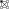
\includegraphics[align=c,scale=1]{flags/k4} or
\includegraphics[align=c,scale=0.75]{pop_sum_graph}.

The study of graphs (Graph Theory) has been a central pillar of mathematics since Euler studied the
bridges of Königsberg in 1736. One of the first things we can study is the fact
that graphs can contain other graphs: Take some subset of the vertices
and look at only those vertices and the edges between them and you end up with another graph.
One can then ask, "How many copies of a graph $F$ are there in a graph $G$"?
A famous Dutch result is \textit{Mantel's theorem} which says a graph of size $n$
with no triangles ($\triangleflag$) has $\leq \frac{n^2}{4}$ edges.

We can then ask, "What is the \textit{density} of a graph $F$ in another graph $G$"? i.e. How
many copies of $F$ are there in $G$, divided by by the max possible number of copies of $F$.
We call this $p(F; G)$.
Consider a graph with $n$ vertices and $m$ edges:
There are at most $\binom{n}{2}$ edges in a graph of size $n$, so we say the \textit{edge
density} is $p(\edge; G) = m/\binom{n}{2}$.
We can re-write Mantel's
theorem to say the density of edges in a triangle free graph is at most
$m/\binom{n}{2} \leq \frac{n^2}{4}/\binom{n}{2} \approx \frac{1}{2}$.
It turns out these densities have some
nice properties. For example, in any graph the density of edges (\edge) and non-edges
(\nonedge) always add up to 1. This is as the number of pairs of vertices which don't have
an edge is $\binom{n}{2} - m$ hence:
\[p(\edge; G) + p(\nonedge; G) = \frac{m}{\binom{n}{2}}+\frac{\binom{n}{2}-m}{\binom{n}{2}} = 1\]

In general, the sum of the densities of all graphs of some fixed size
is always 1! If we wanted to come up with some nice notation to work with we might like to write
this as $\edge + \nonedge = 1$,
$\triangleflag + \triangletwoedge + \triangleoneedge + \triangleempty = 1$, etc.
It turns out then that we can rigorously create this notation (formally an algebra)
out of graphs where statements like
$\edge + \nonedge = 1$ are true. Then, any statement we prove with this notation turns out
to be a true statement about densities of graphs. These algebras are called \textit{flag algebras}.
These algebras are very easily manipulated by computers so we can use them in combination
with computer search to prove new results about densities.

In this thesis we create a new type of algebra very similar to flag algebras which we
use to make progress on some classic graph theory problems, as well as some new problems.

One classic problem we made progress on is the \textit{strong edge colouring conjecture}:
Given a graph we can assign a colour to each edge. A \textit{proper} colouring is one where
no edges which touch (share a vertex) have the same
colour. A \textit{strong} colouring then also requires edges which touch a common edge
have different colours. We can then ask "What is the minimum colours needed for a
strong edge colouring"?
Erd\H{o}s and Nešetřil conjectured in 1985 that you only need $1.25\Delta(G)^2$ colours
where $\Delta(G)$ is the max degree (the max number of edges at any vertex). We prove,
using our local flags, that you need at most $1.73\Delta(G)^2$ colours,
which is the best known bound.

\begin{figure}[!ht]
    \centering
    \includegraphics[scale=1.25]{proper-strong-example}\par
    Non-proper, proper and strong edge colourings.
\end{figure}

\restoregeometry

\appendix

\chapter{Notation}
\label{app:notation}
\begin{itemize}
    \item $[k]:$ The set $\{1, \dots, k\}\subseteq\N.$ $[0]=\emptyset.$
    \item $G[U]:$ Induced subgraph.
    \item $|\sigma|, |F|:$ The type size and flag size (number of vertices) respectively.
    \item $\cong:$ Isomorphism.
    \item $N_G(v):$ The neighbourhood of $v$ in $G$ (subscript often omitted).
    \item $a := b:$ Define $a$ to be equal to $b.$
    \item $\im f:$ The image of a function $f$.
    \item $X \succ 0$: $X$ is positive semidefinite.
    \item $\coef_j$: Coefficient function. Only well defined relative to some ordered basis.
    \item $G^v$ for $v\in V(G)$ is the $\vertex$-flag where $v$ is labelled.
    \item $\emptyset$: Can denote the empty set or the empty graph.
    \item $\binom{X}{k}$: for $X$ a set is the set of $k$-subsets of $X$.
\end{itemize}
We use the following asymptotic notation:\footnote{We tend to write $f\in O(g(n))$ where it is more
customary to write $f = O(g(n))$. This is as we prefer to avoid ``one way equalities'', this is just
notational convention.}
\begin{itemize}
    \item $f(n) \in O(g(n))$ means $\exists k> 0, \exists N$ such that $f(n) \leq kg(n)\ \forall\
        n\geq N$. Alternatively $\limsup_{n\to\infty}\frac{f(n)}{g(n)} < \infty$.
    \item $f(n) \in o(g(n))$ means $\lim_{n\to\infty} \frac{f(n)}{g(n)} = 0$.
    \item $f(n) \in \Omega(g(n))$ means $\exists k> 0, \exists N$ such that $f(n) \geq kg(n)\ \forall\
        n\geq N$. Alternatively $\liminf_{n\to\infty}\frac{f(n)}{g(n)} > 0$.
    \item $f(n) \in \omega(g(n))$ means $\lim_{n\to\infty} \frac{f(n)}{g(n)} = \infty$.
    \item $f(n) \in \Theta(g(n))$ means $f\in O(g(n))$ and $f\in \Omega(n)$.
    \item $f(n) \sim g(n)$ means $f=(1+o(1))g(n)$.
\end{itemize}

\chapter{Software Implementation}
\label{app:flag_software}

Our implementations of the SDP programs are built on the flag software written by
Rémi de Verclos. In particular there are the following two projects:
\begin{itemize}
    \item An implementation of the classic flag algebras based on work done during his
        PhD (\cite{deverclosApplicationsLimitsCombinatorial2016})
        \url{https://github.com/avangogo/rust-flag-algebra}.
    \item A library using the previous implementation written to test if the local flags idea
        would work in principle: \url{https://github.com/avangogo/local-flags}.
\end{itemize}

The modifications made to these projects for this thesis can be found in the following forks:
\url{https://github.com/EoinDavey/rust-flag-algebra} and\\
\url{https://github.com/EoinDavey/local-flags}.
These implementations use Rust\footnote{\url{https://www.rust-lang.org/}} to generate SDP programs which are
then solved using CSDP\footnote{\url{https://github.com/coin-or/Csdp/wiki}},
a standard open source SDP solver
\cite{borchersCSDPLibrarySemidefinite1999}.

\begin{note*}
    Rust is a good choice of language for this application. It is a strongly, statically typed
    language with high level constructions meaning we can define concepts such as flags, types
    etc directly in the code. It is however also extremely fast, meaning the bulk computation
    of matrices of coefficients over large bases is still extremely fast.
\end{note*}

The implementations for the applications in this thesis can be found at these locations:
\begin{itemize}
    \item The "direct" pentagon bounding result, lemma
        \ref{lemma:pentagon_1_4_bound}:\\
        \verb|local-flags/examples/bounded_pentagon.rs|.
    \item The stronger pentagon bounding result, lemma
        \ref{lemma:pentagon_stronger_bound}:\\
        \verb|local-flags/examples/bounded_pentagon_alt_approach.rs|.
    \item The strong edge colouring conjecture bound, lemma
        \ref{lemma:sec_sdp_soln}:\\
        \verb|local-flags/examples/strong_density.rs|.
    \item The bipartite strong edge colouring conjecture bound, lemma
        \ref{lemma:sec_bipartite_sdp_soln}:\\
        \verb|local-flags/examples/bipartite_strong_density.rs|.
\end{itemize}

\noindent At an extremely high level, the local flag algebra programs do the following steps:
\begin{enumerate}
    \item Define the class of local $\emptyset$-flags by defining a sub-class of
        coloured graphs.
    \item Compute an ordered basis of flags of fixed size $n$.
    \item Construct the objective vector over this basis.
    \item Enumerate linear constraint vectors over this basis.
    \item Calculate all local types $\sigma$ and sizes $k$ such that $f^2$ is a vector
        of size $n$ if $f \in \Lcl^\sigma_m$. Generate the coefficient matrices
        $C^\sigma_i$ as described in section \ref{sec:semidefinite_method}.
    \item Write all these vectors and matrices in standard format (SDPA Sparse) such that it
        can be used with CSDP.
    \item Call CSDP as a subroutine to solve the generated SDP problem.
    \item (Optionally) read the generated SDP solution and generate a HTML report.
\end{enumerate}

After these programs have completed and found an optimal bound for the SDP
they will create a \textit{certificate} file containing the optimal (dual and primal)
solution in SDPA-Sparse format. This certificate contains the linear coefficients
and PSD matrices needed to extract a rigorous proof that $\lambda\emptyset - O\in\SemCone^\emptyset$
where $\lambda$ is our optimal bound and $O$ is the objective vector. We give more
information on recovering the proof in appendix \ref{app:sdp_verification}.

\section*{Example}

We show now some of the details of how the proof of lemma \ref{lemma:pentagon_1_4_bound}
is implemented. I'll skip all boilerplate and show only the code which is of high
importance:

First we have some code describing the local $\emptyset$-flags which are those
where each connected component contains a black vertex and there are no
triangles or edges between black vertices.

\begin{lstlisting}[basicstyle=\scriptsize, language=rust]
impl SubFlag<G> for TriangleFreeConnected {
    const HEREDITARY: bool = false;

    fn is_in_subclass(flag: &G) -> bool {
        // Each connected component contains a vertex colored 0
        if !flag.is_connected_to(|i| flag.color[i] == 0) {
            return false;
        }
        // No black-black edges.
        if flag.content.edges()
            .any(|(u, v)| flag.color[u] == 0 && flag.color[v] == 0) {
            return false;
        }
        // No triangles.
        let n = flag.content.size();
        for (u, v, w) in iproduct!(0..n, 0..n, 0..n) {
            if u == v || u == w || v == w {
                continue;
            }
            if !flag.content.edge(u, v)
                || !flag.content.edge(u, w)
                || !flag.content.edge(v, w) {
                continue;
            }
            return false;
        }
        true
    }
}
\end{lstlisting}

We then create the basis of flags of size 5 and construct our
objective vector $O=\llbracket \brrb \cdot \ext_1^\sigma \rrbracket$.
We use a helper function \verb|Degree::project| to construct the extension vectors.

\begin{lstlisting}[basicstyle=\scriptsize, language=rust]
pub fn main() {
    let n = 5;
    let basis = Basis::new(n);

    let c5_path: F = Colored::new(
            Graph::new(4, &[(0, 1), (1, 2), (2, 3)]), vec![0, 1, 1, 0])
            .into();
    let obj = Degree::project(&c5_path, n).untype();
    ...
}
\end{lstlisting}

Then we create a vector of inequalities, which we fill with the inequalities
meaning $\phi(F) \geq 0$ for all flags, $\phi(\llbracket B_k \cdot \ext^{B_k}_1 \rrbracket) = 1$
and the regularity constraints
$\phi(\llbracket \ext_i^\sigma - \ext_j^\sigma\rrbracket) = 0$.
\begin{lstlisting}[basicstyle=\scriptsize, language=rust]
let mut ineqs = vec![flags_are_nonnegative(basis)];
for i in 1..=n {
    ineqs.push(ones(n, i).untype().equal(1.));
}

ineqs.append(&mut Degree::regularity(basis));
\end{lstlisting}

Finally we construct a \verb|Problem| object with these linear constraints and
all $\phi(\llbracket f^2\rrbracket) \geq 0$ constraints\footnote{These are referred to
as Cauchy-Schwarz inequalities in the codebase}.
We then use the convenience object \verb|FlagSolver| to execute this problem
and to print a HTML report.

\begin{lstlisting}[basicstyle=\scriptsize, language=rust]
let pb = Problem::<N, _> {
    ineqs,
    cs: basis.all_cs(),
    obj: -obj,
}
.no_scale(); // Means we don't have to rescale the output.

let mut f = FlagSolver::new(pb, "bounded_pentagon");
f.init();
f.print_report(); // Write some informations in report.html
\end{lstlisting}

Executing this code with \verb|cargo run --release --example bounded_pentagon|\\
prints output \verb|Optimal value: 0.25000001| which is $1/4$ up to floating point error
as expected. The program writes the dual and primal solutions to disk as a file
\verb|certificate|, and the HTML report as \verb|report.html|.

The report should allow a quick visual check that the flag vectors look as expected.
This is most useful for small $n$, as for large $n$ the flags vectors are too large.

\begin{note*}
    The programs generate a lot of precomputed data which is stored locally in a
    directory \verb|data/|. This can be quite a large amount of data, so users should
    take care to not run flag programs for $n$ too large unchecked, as they could in
    theory use up all disk space.
\end{note*}

\section*{Notes on Correctness}

There are a few features and properties of the flag-algebra library which are valid
to use for classic flag algebras, but either are not valid for local flags or
we did not prove that they were valid.
\begin{itemize}
    \item Some operations in the flag-algebra library assume that the sum of flags
        of a fixed size is always equal to 1, which is not true for local flags.
        Having\\
        \verb|HEREDITARY = false| in the graph class definition should disable
        these operations.
    \item The \verb|rust-flag-algebra| library as written by de Verclos has some behaviour where it
        modifies some of the Cauchy-Schwarz matrices. I could not identify why it does
        this but I think it was intended to reduce the size of the generated SDP
        programs by taking advantage of some invariants across flags. As I could not validate what
        this behaviour was doing I disabled it in my fork of this library. Hence it is important
        (unless you can identify what these modifications are doing) to use the modified
        version of the \verb|rust-flag-algebra| library.
    \item There is a function \verb|multiply_and_unlabel| in the \verb|rust-flag-algebra|
        library which I did not prove was correct for local flags, but I suspect it is.
\end{itemize}


\printbibliography{}

\end{document}
